% !TeX root = ../../Book5.tex
% 纲要标题：## 第17章　Weyl 群、Dynkin 图与分类
% 纲要位置：工作记录/计划纲要.md，第 4613 行。

\chapter{Weyl 群、Dynkin 图与分类}
\label{b5:ch:17}
\BookChapterNumber{b5:ch:17}

\begin{chapterabstract}
本章研究 Weyl 群的长度与 Weyl 室、支配权和 Dynkin 图，分类有限约化结晶根系，并以 Serre 展示建立相应复半单 Lie 代数的存在与唯一性。
\end{chapterabstract}

\begin{learninggoals}
\begin{itemize}
\item 能计算简单反射和 Weyl 群长度，用逐次反射求支配代表，并区分根格与权格。
\item 能在带箭头的 Dynkin 图与 Cartan 矩阵之间转换，并保持行列约定。
\item 用正定性排除圈、过多分叉与重边，说明根系分类为何穷尽。
\item 能在经典坐标模型及 \(E_8\) 格模型中直接检查根的性质。
\item 在 Serre 构造中，分别检验三角分解的线性生成关系、生成元的非零性、有限维性及半单性。
\end{itemize}
预备知识为\chapref{b5:ch:16}的根系公理、简单根及根弦，以及实正定二次型与整数格。
第17.4节还用自由代数和生成关系的商；其构造在该节回顾。
\end{learninggoals}

在 \(A_2\) 根系中，除两个简单根 \(\alpha_1,\alpha_2\) 外，正根还有 \(\alpha_1+\alpha_2\)。关于 \(\alpha_1\) 的反射把它自身送到负根，却把 \(\alpha_2\) 送到 \(\alpha_1+\alpha_2\)。一次反射既改变了某个根的符号，又在其余正根之间作置换。若反复反射，怎样判断一个表达式已是最短的，怎样从许多 Weyl 室中挑出标准代表？简单根间允许的角度还会限制可出现的图形。本章从这项几何计算进入长度、权室与 Dynkin 图的分类。

% !TeX root = ../../Book5.tex
% 纲要标题：### 17.1 Weyl 群
% 纲要位置：工作记录/计划纲要.md，第 4615 行。

\section{Weyl 群}
\label{b5:sec:1701}

从单个根反射走向它们生成的群，需要同时研究反射乘积和正根符号。交换引理将把最短表达、Weyl 室及支配代表联系起来。

% 纲要要点已在下文展开。

% 纲要细目（保留原定写作范围）：
%
% * 简单反射
% * Weyl 室与长度
% * 权格和根格
% * 用秩二交换计算和逐次反射说明长度与支配代表，用秩一自然表示区分根格与权格
%

\subsection{简单反射}
\label{b5:subsec:1701:01}

\begin{definition}\label{b5:def:weyl-group}
	设 \(E\) 为有限维实内积空间，\(\Phi\subseteq E\) 为有限约化结晶根系，\(s_\alpha\) 为根 \(\alpha\) 对应的正交反射。由这些反射生成的正交变换群称为 \(\Phi\) 的\term{Weyl 群}[Weyl group]，记为 \(W\)。固定简单根基 \(\Delta=\{\alpha_1,\ldots,\alpha_r\}\) 后，记 \(s_i=s_{\alpha_i}\)。
\end{definition}
\symidx{\(W,\Delta\)：根系的 Weyl 群与所选简单根基}

因为 \(W\) 置换有限集合 \(\Phi\)，而 \(\Phi\) 生成 \(E\)，故这个置换作用忠实，\(W\) 是有限群。\cref{b5:prop:simple-reflection-positive}还说明它由简单反射生成：每个根写成 \(w\alpha_i\)，其中 \(w\) 是简单反射的乘积，则 \(s_{w\alpha_i}=ws_iw^{-1}\)。

\begin{lemma}[删去一个反射]\label{b5:lem:weyl-exchange}
	设 \(\Phi\subseteq E\) 为有限约化结晶根系，选定正根集合及其简单根基 \(\{\alpha_1,\ldots,\alpha_r\}\)，记 \(s_i=s_{\alpha_i}\) 为相应简单反射。设 \(w=s_{i_1}\cdots s_{i_m}\)。若 \(w\alpha_j\) 为负根，则 \(ws_j\) 可由所列乘积删去某一个因子得到。
\end{lemma}
\begin{proof}
	从右向左依次把各反射作用于 \(\alpha_j\)。它起初为正，最终为负，故某一步首次把正根变成负根。 简单反射只把自己的简单根变为负根，因此存在 \(k\)，使
	\[
		v\alpha_j=\alpha_{i_k},\qquad v=s_{i_{k+1}}\cdots s_{i_m}.
	\]
	反射的共轭公式给出 \(vs_jv^{-1}=s_{i_k}\)，故
	\[
		ws_j =s_{i_1}\cdots s_{i_{k-1}}s_{i_k}vs_j =s_{i_1}\cdots s_{i_{k-1}}v.
	\]
	这正是删去第 \(k\) 个因子的乘积。
\end{proof}

在 \(A_2\) 中，简单反射满足 \(s_1\alpha_2=s_2\alpha_1=\alpha_1+\alpha_2\)。取 \(w=s_1s_2s_1\)，从右向左作用于 \(\alpha_2\)，得到
\[
	\alpha_2\xrightarrow{s_1}\alpha_1+\alpha_2 \xrightarrow{s_2}\alpha_1\xrightarrow{s_1}-\alpha_1.
\]
首次变号发生在最左侧的 \(s_1\)，所以交换引理删去原表达的第一个因子，给出
\[
	(s_1s_2s_1)s_2=s_2s_1.
\]
具体地，\(v=s_2s_1\) 满足 \(v\alpha_2=\alpha_1\)，从而 \(vs_2v^{-1}=s_1\)，这正是证明中的消去步骤。删去的因子不必位于原乘积的末端。再在右边乘 \(s_2\)，还得到 \(s_1s_2s_1=s_2s_1s_2\)。

\subsection{Weyl 室与长度}
\label{b5:subsec:1701:02}

全部根超平面 \(H_\alpha=\bigl\{\,x\in E\mid(x,\alpha)=0\,\bigr\}\) 把其补集分成若干连通分支，称为\term{Weyl 室}[Weyl chamber]。 选定简单根所对应的基本室为
\[
	C=\bigl\{\,x\in E\mid(x,\alpha_i)>0\;\text{对所有}\;i\,\bigr\}.
\]
其闭包 \(\overline C=\{x\in E\mid(x,\alpha_i)\ge0\;\text{对所有}\;i\}\) 称为闭基本室，也称闭支配室；属于它的向量称为支配向量。 基本室 \(C\) 确是一个连通分支：正根为简单根的非负整数和，所以 \(C\) 中所有正根的值都为正；它又是若干开半空间的交，因而凸且连通。任何不穿过根超平面的连续路径都不能改变这些符号。

\begin{theorem}\label{b5:thm:weyl-chambers-length}
	设 \(\Phi\subseteq E\) 为有限约化结晶根系，\(E\) 为实内积空间，\(W\) 为其 Weyl 群。选定正根集合 \(\Phi^+\) 及简单根基 \(\{\alpha_1,\ldots,\alpha_r\}\)，令 \(C=\{v\in E\mid(v,\alpha_i)>0\;\text{对所有}\;i\}\) 为基本 Weyl 室，\(\overline C\) 为其闭包。对 \(w\in W\)，令 \(\ell(w)\) 为其最短简单反射乘积的因子数。则
	\begin{equation}\label{b5:eq:weyl-length-inversions}
		\ell(w)=\#\{\,\alpha\in\Phi^+\mid w\alpha\in-\Phi^+\,\}.
	\end{equation}
	此外，\(W\) 在 Weyl 室上单纯传递，每个 \(W\)-轨道与闭基本室 \(\overline C\) 相交于唯一一点。
\end{theorem}
\begin{proof}
	将右边记为 \(N(w)\)。因 \(s_i\) 置换除 \(\alpha_i\) 外的正根，有
	\[
		N(ws_i)=
		\begin{cases}
			N(w)+1,&w\alpha_i>0,\\
			N(w)-1,&w\alpha_i<0.
		\end{cases}
	\]
	对一个最短表达 \(w=us_i\)，其前缀也是最短表达。若 \(u\alpha_i<0\)，\cref{b5:lem:weyl-exchange}会把 \(us_i\) 写成比当前表达少两个因子的乘积，矛盾。因此 \(u\alpha_i>0\)，按长度归纳得到 \(N(w)=\ell(w)\)。

	取 \(c\in C\)。对任意 \(x\in E\)，在有限轨道 \(Wx\) 中选取与 \(c\) 内积最大的 \(y\)。若 \((y,\alpha_i)<0\)，则
	\[
		(s_i y,c)-(y,c) =-\frac{2(y,\alpha_i)(\alpha_i,c)}{(\alpha_i,\alpha_i)}>0,
	\]
	矛盾。所以 \(y\in\overline C\)。若 \(x\) 不在任何根超平面上，则 \(y=wx\) 也不在其中，因为 \(W\) 置换根超平面。因而所有 \((y,\alpha_i)\ge0\) 都不能为零，实际均为正，即 \(y\in C\)。这说明各室均为某个 \(wC\)。 若 \(wC=C\)，则 \(w\) 保持正根，故 \(N(w)=0\)，从而 \(w=1\)。

	还要处理闭室的边界。若 \(w=s_{i_1}\cdots s_{i_m}\) 最短，则每个 \(\beta_k=s_{i_1}\cdots s_{i_{k-1}}\alpha_{i_k}\) 为正根；否则交换引理使相应前缀变短。相邻前缀之差相加，得到算子恒等式
	\[
		1-s_{i_1}\cdots s_{i_m} =\sum_{k=1}^m s_{i_1}\cdots s_{i_{k-1}}(1-s_{i_k}),
	\]
	其中空乘积为恒等算子。将它作用于任意支配向量 \(\mu\in\overline C\)，再用反射公式，得到
	\begin{equation}\label{b5:eq:dominant-weyl-difference}
		\mu-w\mu =\sum_{k=1}^m \frac{2(\mu,\alpha_{i_k})}{(\alpha_{i_k},\alpha_{i_k})}\,\beta_k.
	\end{equation}
	所以 \(\mu-w\mu\) 是简单根的非负实线性组合。若 \(w\mu\) 也支配，反过来用 \(w^{-1}\)，则 \(w\mu-\mu\) 也是这样的组合。简单根线性无关，迫使二者都为零。因此闭室中的代表唯一。
\end{proof}

在 \(A_{n-1}\) 的标准坐标中，\(W=S_n\) 置换坐标；一个基本室由 \(x_1>x_2>\cdots>x_n\)、\(\sum x_i=0\) 给出。 长度公式便成为排列的逆序数公式。坐标相等时，向量落在室的边界上，其稳定子群可以非平凡，这与室内部的单纯传递性并不冲突。

\ProseParagraphBreak

在 \(A_2\) 中，将简单根画成 \(\alpha_1=(1,0)\)、\(\alpha_2=(-1/2,\sqrt3/2)\)。两根之间的角是 \(120^\circ\)，基本室却由它们的垂直墙围成，角为 \(60^\circ\)。从 \(C\) 依次走到 \(s_1C,s_1s_2C,s_1s_2s_1C\)，穿过的墙分别垂直于 \(\alpha_1,\alpha_1+\alpha_2,\alpha_2\)。终点是相反室，三个正根全都变号，长度公式因而给出 \(\ell(s_1s_2s_1)=3\)。这些墙与根的对应画在\cref{b5:fig:a2-chambers-lattices}中；墙上的基本权将在下面给出坐标。

\subsection{权格和根格}
\label{b5:subsec:1701:03}

\begin{definition}\label{b5:def:weight-lattice}
	设 \(E\) 为有限维实内积空间，\(\Phi\subseteq E\) 为有限约化结晶根系，固定简单根基 \(\{\alpha_1,\ldots,\alpha_r\}\)，记 \(\overline C=\{v\in E\mid(v,\alpha_i)\ge0\;\text{对所有}\;i\}\) 为闭基本室。 令 \(\alpha^\vee=2\alpha/(\alpha,\alpha)\)，并记 \(\langle\lambda,\alpha^\vee\rangle=2(\lambda,\alpha)/(\alpha,\alpha)\)。 两个格
	\[
		Q=\sum_i\mathbb Z\alpha_i,\qquad P=\bigl\{\,\lambda\in E\mid \langle\lambda,\alpha^\vee\rangle\in\mathbb Z \;\text{对所有}\;\alpha\in\Phi\,\bigr\}
	\]
	分别称为\term{根格}[root lattice]和\term{权格}[weight lattice]。 满足 \(\langle\omega_i,\alpha_j^\vee\rangle=\delta_{ij}\) 的向量 \(\omega_i\) 称为\term{基本权}[fundamental weight]。 属于 \(P\cap\overline C\) 的向量称为\term{支配整权}[dominant integral weight]，其集合记为 \(P^+\)。
\end{definition}
\symidx{\(\alpha^\vee,\langle\lambda,\alpha^\vee\rangle\)：余根及权与余根的配对}
\symidx{\(Q,P\)：根格与权格}
\symidx{\(\omega_i,P^+\)：基本权与支配整权集合}

\begin{proposition}\label{b5:prop:weight-fundamental-basis}
	设 \(\Phi\subseteq E\) 为有限约化结晶根系，\(\{\alpha_1,\ldots,\alpha_r\}\) 为简单根基，\(\omega_i\) 为相应基本权，即 \(\langle\omega_i,\alpha_j^\vee\rangle=\delta_{ij}\)。记 \(P\) 为权格，\(Q\) 为根格，\(P^+\) 为支配整权集合。则
	\[
		P=\bigoplus_i\mathbb Z\omega_i,\qquad P^+=\sum_i\mathbb Z_{\geq0}\omega_i,\qquad Q\subseteq P,
	\]
	且 \(P/Q\) 有限。检验一个向量是否属于 \(P\)，只须检验它与简单余根的配对是否全为整数。
\end{proposition}
\begin{proof}
	余根集合本身也是根系：反射与原根系相同，结晶整数交换了原来的两个根参数。 若正根 \(\beta=\sum_i c_i\alpha_i\)、\(c_i\ge0\)，则
	\[
		\beta^\vee=\frac{2\beta}{(\beta,\beta)} =\sum_i c_i\frac{(\alpha_i,\alpha_i)}{(\beta,\beta)}\alpha_i^\vee.
	\]
	系数均非负，所以每个正根的余根都是简单余根的非负实组合。若一个简单余根是两个正余根之和，比较在简单余根基下的非负实系数，两个加数都只能在该简单余根的射线上；约化性使它们都等于该简单余根，矛盾。 因此全部简单余根都是余根系的简单根；它们已有 \(r\) 个，由\cref{b5:thm:simple-roots}，正好组成余根系的简单根基。 故每个余根都是简单余根的整数和，检验简化随之成立。 基本权是简单余根的对偶基，所以所列两种展开立即成立。结晶条件给出 \(Q\subseteq P\)。 令 \(A=(a_{ij})\)、\(a_{ij}=\langle\alpha_j,\alpha_i^\vee\rangle\)。由基本权的对偶关系， \(\alpha_j=\sum_i a_{ij}\omega_i\)，故在基本权坐标下 \(P=\mathbb Z^r\)、\(Q=A\mathbb Z^r\)。 矩阵 \(A\) 可逆且为整数矩阵，\(\operatorname{adj}(A)\) 也是整数矩阵；恒等式 \(A\operatorname{adj}(A)=(\det A)I\) 给出 \((\det A)\omega_j\in Q\) 对每个 \(j\) 成立。因此有限群 \(P/(|\det A|P)\) 满射到 \(P/Q\)，后者也有限。
\end{proof}

根格与权格的差别在秩一已经出现。对 \(A_1\) 根系 \(\Phi=\{\alpha,-\alpha\}\)，基本权为 \(\omega=\dfrac{\alpha}{2}\)，因为 \(\langle\omega,\alpha^\vee\rangle=1\)。于是
\[
	\begin{aligned}
		Q&=\mathbb Z\alpha=2\mathbb Z\omega,\qquad P=\mathbb Z\omega,\\
		P/Q&\cong\mathbb Z/2\mathbb Z,\qquad P^+=\mathbb Z_{\ge0}\omega.
	\end{aligned}
\]

\ProseParagraphBreak

这个额外的半根在表示中确实出现。对 \(\mathfrak{sl}_2(\mathbb C)\)，取标准基 \(e,f,h\)，正根满足 \(\alpha(h)=2\)；\cref{b5:thm:root-sl2}中的余根元 \(h_\alpha\) 在这里就是 \(h\)。自然二维模 \(L_1\) 的最高向量 \(v\) 满足 \(ev=0\)、\(hv=v\)，故其最高权 \(\lambda\) 满足 \(\lambda(h)=1\)，即 \(\lambda=\omega=\dfrac{\alpha}{2}\notin Q\)。更一般地，\cref{b5:prop:sl2-model,b5:thm:sl2-classification}中的 \(L_m\) 以 \(hv_0=mv_0\) 给出最高权 \(m\omega\)，所以这些有限维不可约模的最高权恰好取遍 \(P^+\)。根格记录根的整数和，权格则容纳了这些并非都在根格中的最高权。

\ProseParagraphBreak

正简单根实锥与闭支配室使用两套非负条件。若 \(K=\sum_i\mathbb R_{\ge0}\alpha_i\)，则
\[
	\overline C=\{\,x\in E\mid(x,y)\ge0\;\text{对所有}\;y\in K\,\},
\]
所以闭支配室是 \(K\) 的内积对偶锥。在上述 \(A_2\) 坐标中，配对方程给出
\[
	\omega_1=(1/2,\sqrt3/6),\qquad \omega_2=(0,\sqrt3/3), \qquad \alpha_1=2\omega_1-\omega_2,\quad \alpha_2=-\omega_1+2\omega_2.
\]
因此正根 \(\alpha_2\) 不是支配权，而 \(\omega_1\) 是支配整权却不在根格中：由两式解得 \(\omega_1=(2\alpha_1+\alpha_2)/3\)，其简单根系数不是整数。又有 \((\omega_1,\alpha_2)=0\)，故 \(s_2\omega_1=\omega_1\)。图中的格点及墙同时展示了这些区别；边界点有稳定子群，不影响开室集合上的单纯传递作用。

% !TeX root = ../Book5.tex
\begin{figure}[htbp]
	\centering
	\begin{tikzpicture}[x=2.7cm,y=2.7cm,every node/.style={font=\small}]
		\fill[yellow!12] (0,0)--(0:1.18) arc[start angle=0,end angle=120,radius=1.18]--cycle;
		\fill[AlgebraBlue!12] (0,0)--(30:1.18) arc[start angle=30,end angle=90,radius=1.18]--cycle;
		\foreach \m in {-3,...,3} {
			\foreach \n in {-3,...,3} {
				\pgfmathsetmacro{\px}{\m/2}
				\pgfmathsetmacro{\py}{sqrt(3)*(\m/6+\n/3)}
				\pgfmathtruncatemacro{\inside}{(\px*\px+\py*\py<2.35)?1:0}
				\ifnum\inside=1
					\fill[gray!45] (\px,\py) circle[radius=.6pt];
					\pgfmathtruncatemacro{\rootpoint}{mod(\m+2*\n,3)}
					\ifnum\rootpoint=0
						\fill[black] (\px,\py) circle[radius=1.1pt];
					\fi
				\fi
			}
		}
		\foreach \angle in {30,90,150} {
			\draw[dashed,gray] (\angle:1.60)--(\angle+180:1.60);
		}
		\foreach \angle/\name in {0/\alpha_1,60/{\alpha_1+\alpha_2},120/\alpha_2,
			180/{-\alpha_1},240/{-\alpha_1-\alpha_2},300/{-\alpha_2}} {
			\draw[->,line width=.7pt] (0,0)--(\angle:1);
			\node[fill=white,inner sep=1pt] at (\angle:1.17) {\(\name\)};
		}
		\draw[->,AlgebraBlue,line width=.9pt] (0,0)--(.5,.288675);
		\draw[->,AlgebraBlue,line width=.9pt] (0,0)--(0,.577350);
		\node[anchor=north west,text=AlgebraBlue] at (.5,.288675) {\(\omega_1\)};
		\node[anchor=east,text=AlgebraBlue] at (0,.577350) {\(\omega_2\)};
		\node[anchor=north east] at (0,0) {\(0\)};
		\foreach \angle in {60,120,180} {
			\draw[->,AlgebraBlue,line width=.7pt]
				(\angle:1.48) arc[start angle=\angle,end angle=\angle+55,radius=1.48];
		}
		\node at (60:1.73) {\(C\)};
		\node at (120:1.73) {\(s_1C\)};
		\node at (180:1.85) {\(s_1s_2C\)};
		\node at (240:1.75) {\(s_1s_2s_1C=-C\)};
	\end{tikzpicture}
	\caption[\(A_2\) 的室与两种格]{\(A_2\) 的六根、三条墙及室链。 淡黄色扇形是正简单根实锥，蓝色扇形是基本室；二者的边界不同。 灰点表示权格，黑点表示根格。\(\omega_1\) 位于垂直于 \(\alpha_2\) 的墙上，故被 \(s_2\) 固定。 外侧箭头给出到相反室的三步最短室链。}
	\label{b5:fig:a2-chambers-lattices}
\end{figure}


\begin{proposition}\label{b5:prop:weyl-dominant-order}
	设 \(\Phi\subseteq E\) 为有限约化结晶根系，\(\{\alpha_1,\ldots,\alpha_r\}\) 为所选简单根基，\(W\) 为 Weyl 群，\(P\) 为权格，\(P^+\) 为支配整权集合。每个 \(\mu\in P\) 的 \(W\) 轨道都有唯一支配整权。若 \(\mu\in P^+\)、\(w\in W\)，则 \(\mu-w\mu\in\sum_i\mathbb Z_{\geq0}\alpha_i\)。
\end{proposition}
\begin{proof}
	反射公式说明 \(W\) 保持 \(P\)，故闭室代表仍为整权。存在唯一性已经由\cref{b5:thm:weyl-chambers-length}证明。公式\eqref{b5:eq:dominant-weyl-difference}中的系数此时都是非负整数，而 \(\beta_k\) 为正根，故给出后一结论。
\end{proof}

\begin{proposition}\label{b5:prop:rho-coroot}
	设 \(\Phi\subseteq E\) 为有限约化结晶根系，\(\Phi^+\) 为所选正根集合，\(\{\alpha_1,\ldots,\alpha_r\}\) 为相应简单根基，\(\omega_i\) 为基本权，\(\alpha_i^\vee\) 为简单余根。令 \(\rho=\dfrac12\sum_{\alpha\in\Phi^+}\alpha\)。则 \(\rho=\sum_i\omega_i\)，特别地 \(\langle\rho,\alpha_i^\vee\rangle=1\)。
\end{proposition}
\symidx{\(\rho=\frac12\sum_{\alpha\in\Phi^+}\alpha\)：正根和的一半}
\begin{proof}
	\(s_i\) 置换除 \(\alpha_i\) 外的正根，故 \(s_i\rho=\rho-\alpha_i\)。 与反射公式比较便得每个配对等于 \(1\)，再用基本权基展开。
\end{proof}

支配代表也可以逐步求出。对任意 \(\mu\in P\)，从 \(\mu_0=\mu\) 开始；若当前有 \(\langle\mu_k,\alpha_i^\vee\rangle<0\)，便任选这样的 \(i\)，令
\[
	\mu_{k+1}=s_i\mu_k =\mu_k-\langle\mu_k,\alpha_i^\vee\rangle\alpha_i.
\]
固定 \(c\in C\)，每一步都满足
\[
	(\mu_{k+1},c)-(\mu_k,c) =-\langle\mu_k,\alpha_i^\vee\rangle(\alpha_i,c)>0.
\]
所有 \(\mu_k\) 都在有限轨道 \(W\mu\) 中，严格增加使任何点都不能重复，故至多经过 \(\#(W\mu)-1\) 次反射便终止。终止时所有简单余根配对非负，且反射始终保持权格，所以所得点属于 \(P^+\)；\cref{b5:prop:weyl-dominant-order}保证它是唯一的支配代表。

\ProseParagraphBreak

例如在 \(A_2\) 中，\(\rho=\alpha_1+\alpha_2=\omega_1+\omega_2\)。从 \(-\rho\) 出发，先选 \(s_1\)，再依次选 \(s_2,s_1\)，有
\[
	-\rho\xrightarrow{s_1}-\alpha_2 \xrightarrow{s_2}\alpha_2\xrightarrow{s_1}\rho.
\]
各点与 \((\alpha_1^\vee,\alpha_2^\vee)\) 的配对依次为
\[
	(-1,-1),\qquad(1,-2),\qquad(-1,2),\qquad(1,1).
\]
每次选用的反射都对应一个负配对；最后两个配对均为正，过程到达基本室内部。

% !TeX root = ../../Book5.tex
% 纲要标题：### 17.2 Cartan 矩阵与 Dynkin 图
% 纲要位置：工作记录/计划纲要.md，第 4622 行。

\section{Cartan 矩阵与 Dynkin 图}
\label{b5:sec:1702}

简单根数目有限，但其内积最初看似仍有连续参数。结晶整数把角度和长度比限制为少数可能，Cartan 矩阵由此成为一份离散的记录。

% 纲要要点已在下文展开。

% 纲要细目（保留原定写作范围）：
%
% * 简单根夹角和长度
% * Cartan 矩阵
% * Dynkin 图的构造
% * 将边重数与反射乘积的阶相联系，以 B3、C3 区分归一化 Gram 数据和长短根方向
%

\subsection{简单根夹角和长度}
\label{b5:subsec:1702:01}

两个不成比例的根 \(\alpha,\beta\) 给出的整数
\[
	a=\frac{2(\beta,\alpha)}{(\alpha,\alpha)},\qquad b=\frac{2(\alpha,\beta)}{(\beta,\beta)}
\]
满足 \(ab=4\cos^2\theta<4\)。对不同简单根，\(a,b\leq0\)，所以可能的有序数对只有
\[
	(0,0),\quad(-1,-1),\quad(-1,-2),\quad(-2,-1), \quad(-1,-3),\quad(-3,-1).
\]
它们对应夹角 \(90^\circ,120^\circ,135^\circ,150^\circ\)； 非等长时，平方长度之比为 \(2\) 或 \(3\)。 这说明结晶条件不仅限制角度，也限制不同长度的相对比例。

\subsection{Cartan 矩阵}
\label{b5:subsec:1702:02}

\begin{definition}\label{b5:def:root-cartan-matrix}
	设 \(\Delta=\{\alpha_1,\ldots,\alpha_r\}\) 为有限约化结晶根系的简单根基。矩阵
	\[
		A=(a_{ij}),\qquad a_{ij}=\langle\alpha_j,\alpha_i^\vee\rangle =\frac{2(\alpha_i,\alpha_j)}{(\alpha_i,\alpha_i)}
	\]
	称为根系的\term{Cartan 矩阵}[Cartan matrix]。本书的行对应余根，列对应根。
\end{definition}
\symidx{\(A=(a_{ij})\)：根系的 Cartan 矩阵}

这个矩阵与模表示论中由投射覆盖重数定义的 Cartan 矩阵是不同对象。这里 \(a_{ii}=2\)，非对角元为非正整数，且 \(a_{ij}=0\) 当且仅当 \(a_{ji}=0\)。 令 \(d_i=(\alpha_i,\alpha_i)/2\)，则 \(\operatorname{diag}(d_i)A\) 是简单根的 Gram 矩阵，故对称正定。特别地 \(A\) 可逆。

\begin{proposition}\label{b5:prop:cartan-determines-roots}
	设两个有限约化结晶根系具有相同的带编号 Cartan 矩阵。把一组简单根送到另一组简单根的线性同构，将全部根双射到全部根；在每个不可约分支上，它将内积乘以一个正数。
\end{proposition}
\begin{proof}
	在简单根基下， \(s_i(\alpha_j)=\alpha_j-a_{ij}\alpha_i\)，所以这个线性同构交织全部简单反射。 每个根都是某个简单根经这些反射所得，故它将根集合双射到根集合。 在相邻顶点处，\(a_{ij}/a_{ji}\) 决定平方长度之比；沿连通图传播，所有长度只差一个共同正比例。再由 Cartan 系数恢复全部内积，便得到最后的断言。
\end{proof}

\subsection{Dynkin 图的构造}
\label{b5:subsec:1702:03}

为每个简单根画一个顶点；顶点 \(i,j\) 之间画 \(a_{ij}a_{ji}\) 条边，若是双边或三边，则箭头指向较短的根。所得有向重图称为 Dynkin 图。它同时记录角度及长短，因而恢复 Cartan 矩阵。例如
\[
	A_2:\ \begin{pmatrix}2&-1\\-1&2\end{pmatrix},\qquad
	B_2:\ \begin{pmatrix}2&-1\\-2&2\end{pmatrix},\qquad
	G_2:\ \begin{pmatrix}2&-3\\-1&2\end{pmatrix}.
\]
在这里的 \(B_2\) 编号中第一根长、第二根短；\(G_2\) 的第一根短。 若只保留边数而忘掉箭头，就不能区分一般秩的 \(B_r\) 与 \(C_r\)。

\begin{proposition}\label{b5:prop:dynkin-reflection-order}
	设 \(\Phi\subseteq E\) 为有限约化结晶根系，\(E\) 为实内积空间，\(\{\alpha_1,\ldots,\alpha_r\}\) 为简单根基，\(s_i=s_{\alpha_i}\) 为简单反射，\(A=(a_{ij})\) 为行对应余根、列对应根的 Cartan 矩阵。对 \(i\ne j\)，若 \(a_{ij}a_{ji}\) 分别为 \(0,1,2,3\)，则 \(s_is_j\) 的阶分别为 \(2,3,4,6\)。因而 Dynkin 图中两顶点之间的边数决定这两个反射乘积的阶，箭头不影响这个阶。
\end{proposition}
\begin{proof}
	令 \(U=\operatorname{span}_{\mathbb R}\{\alpha_i,\alpha_j\}\)。两个反射都在 \(U^\perp\) 上恒等。在 \(U\) 中选取正交单位基，使两根的单位方向分别为 \((1,0)\)、\((\cos\theta,\sin\theta)\)，其中 \(0<\theta<\pi\)。由正交反射公式，
	\[
		\begin{aligned}
			s_i\big|_U&=\begin{pmatrix}-1&0\\0&1\end{pmatrix},\qquad
			s_j\big|_U=
			\begin{pmatrix}
				-\cos2\theta&-\sin2\theta\\
				-\sin2\theta&\cos2\theta
			\end{pmatrix},\\
			(s_is_j)\big|_U&=
			\begin{pmatrix}
				\cos2\theta&\sin2\theta\\
				-\sin2\theta&\cos2\theta
			\end{pmatrix}.
		\end{aligned}
	\]
	所以乘积在根平面上是旋转。前面的结晶整数计算给出 \(\theta=90^\circ,120^\circ,135^\circ,150^\circ\)，对应旋转的阶恰为 \(2,3,4,6\)。在正交补上的恒等作用不改变这个阶。
\end{proof}

例如 \(A_2\) 的单边给出 \((s_1s_2)^3=1\)，结合 \(s_1^2=s_2^2=1\)，便得 \(s_1s_2s_1=s_2s_1s_2\)，与交换引理后的计算一致；\(B_2\) 的双边和 \(G_2\) 的三边分别给出乘积阶 \(4\) 和 \(6\)。这里计算了两两反射满足的关系，要证明这些关系给出整个 Weyl 群的完整展示，还需要另外的论证。

\ProseParagraphBreak

有限根系的经典族与例外型的 Dynkin 图分别见\cref{b5:fig:classical-dynkin-diagrams,b5:fig:exceptional-dynkin-diagrams}。 图中的编号与下一节的坐标简单根一致。

% !TeX root = ../Book5.tex
\begin{figure}[htbp]
	\centering
	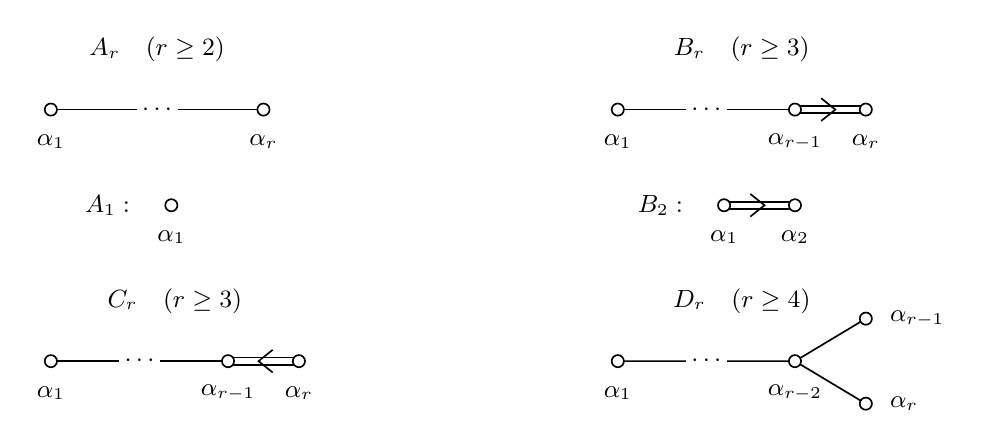
\begin{tikzpicture}[
		x=0.9cm,y=0.9cm,every node/.style={font=\small},
		every path/.style={line width=.6pt},
		root/.style={circle,draw,fill=white,inner sep=0pt,minimum size=4.4pt}]
		% A_r: the omitted single-edge chain may have no intermediate vertices.
		\node at (1.5,0.85) {\(A_r\quad(r\geq2)\)};
		\draw (0,0)--(3,0);
		\node[fill=white,inner sep=2pt] at (1.5,0) {\(\cdots\)};
		\node[root] at (0,0) {};
		\node[root] at (3,0) {};
		\node at (0,-0.45) {\(\alpha_1\)};
		\node at (3,-0.45) {\(\alpha_r\)};
		\node at (0.8,-1.35) {\(A_1:\)};
		\node[root] at (1.7,-1.35) {};
		\node at (1.7,-1.8) {\(\alpha_1\)};

		% B_r: alpha_r is short, so the double-edge arrow points right.
		\node at (9.75,0.85) {\(B_r\quad(r\geq3)\)};
		\draw (8,0)--(10.5,0);
		\node[fill=white,inner sep=2pt] at (9.25,0) {\(\cdots\)};
		\draw (10.5,0.05)--(11.5,0.05) (10.5,-0.05)--(11.5,-0.05);
		\draw (10.87,0.16)--(11.07,0)--(10.87,-0.16);
		\foreach \x in {8,10.5,11.5} \node[root] at (\x,0) {};
		\node at (8,-0.45) {\(\alpha_1\)};
		\node at (10.5,-0.45) {\(\alpha_{r-1}\)};
		\node at (11.5,-0.45) {\(\alpha_r\)};
		\node at (8.6,-1.35) {\(B_2:\)};
		\draw (9.5,-1.3)--(10.5,-1.3) (9.5,-1.4)--(10.5,-1.4);
		\draw (9.87,-1.19)--(10.07,-1.35)--(9.87,-1.51);
		\foreach \x in {9.5,10.5} \node[root] at (\x,-1.35) {};
		\node at (9.5,-1.8) {\(\alpha_1\)};
		\node at (10.5,-1.8) {\(\alpha_2\)};

		% C_r: alpha_r is long, so the double-edge arrow points left.
		\node at (1.75,-2.7) {\(C_r\quad(r\geq3)\)};
		\draw (0,-3.55)--(2.5,-3.55);
		\node[fill=white,inner sep=2pt] at (1.25,-3.55) {\(\cdots\)};
		\draw (2.5,-3.5)--(3.5,-3.5) (2.5,-3.6)--(3.5,-3.6);
		\draw (3.13,-3.39)--(2.93,-3.55)--(3.13,-3.71);
		\foreach \x in {0,2.5,3.5} \node[root] at (\x,-3.55) {};
		\node at (0,-4) {\(\alpha_1\)};
		\node at (2.5,-4) {\(\alpha_{r-1}\)};
		\node at (3.5,-4) {\(\alpha_r\)};

		% D_r: alpha_{r-2} is the fork; at r=4 the omitted chain is one edge.
		\node at (9.75,-2.7) {\(D_r\quad(r\geq4)\)};
		\draw (8,-3.55)--(10.5,-3.55)
			(10.5,-3.55)--(11.5,-2.95) (10.5,-3.55)--(11.5,-4.15);
		\node[fill=white,inner sep=2pt] at (9.25,-3.55) {\(\cdots\)};
		\foreach \x/\y in {8/-3.55,10.5/-3.55,11.5/-2.95,11.5/-4.15}
		\node[root] at (\x,\y) {};
		\node at (8,-4) {\(\alpha_1\)};
		\node at (10.5,-4) {\(\alpha_{r-2}\)};
		\node[anchor=west] at (11.7,-2.95) {\(\alpha_{r-1}\)};
		\node[anchor=west] at (11.7,-4.15) {\(\alpha_r\)};
	\end{tikzpicture}
	\caption[经典型 Dynkin 图]{经典型 Dynkin 图。省略号表示可含零个中间顶点的单边链段，根的编号沿链递增。 双边箭头指向短根；\(D_r\) 的分叉点为 \(\alpha_{r-2}\)。}
	\label{b5:fig:classical-dynkin-diagrams}
\end{figure}

% !TeX root = ../Book5.tex
\begin{figure}[htbp]
	\centering
	\begin{tikzpicture}[
		x=0.9cm,y=0.9cm,every node/.style={font=\small},
		every path/.style={line width=.6pt},
		root/.style={circle,draw,fill=white,inner sep=0pt,minimum size=4.4pt}]
		% E_6, E_7, E_8 use the coordinate-model numbering; alpha_4 is the fork.
		\node at (2,2.05) {\(E_6\)};
		\draw (0,0)--(4,0) (2,0)--(2,1);
		\foreach \x/\i in {0/1,1/3,2/4,3/5,4/6} {
			\node[root] at (\x,0) {};
			\node at (\x,-0.45) {\(\alpha_\i\)};
		}
		\node[root] at (2,1) {};
		\node at (2,1.45) {\(\alpha_2\)};

		\node at (9.5,2.05) {\(E_7\)};
		\draw (7,0)--(12,0) (9,0)--(9,1);
		\foreach \x/\i in {7/1,8/3,9/4,10/5,11/6,12/7} {
			\node[root] at (\x,0) {};
			\node at (\x,-0.45) {\(\alpha_\i\)};
		}
		\node[root] at (9,1) {};
		\node at (9,1.45) {\(\alpha_2\)};

		\node at (6,-1.7) {\(E_8\)};
		\draw (3,-3.55)--(9,-3.55) (5,-3.55)--(5,-2.55);
		\foreach \x/\i in {3/1,4/3,5/4,6/5,7/6,8/7,9/8} {
			\node[root] at (\x,-3.55) {};
			\node at (\x,-4) {\(\alpha_\i\)};
		}
		\node[root] at (5,-2.55) {};
		\node at (5,-2.1) {\(\alpha_2\)};

		% F_4: alpha_1 and alpha_2 are long; alpha_3 and alpha_4 are short.
		\node at (1.5,-5.1) {\(F_4\)};
		\draw (0,-5.95)--(1,-5.95) (2,-5.95)--(3,-5.95);
		\draw (1,-5.9)--(2,-5.9) (1,-6)--(2,-6);
		\draw (1.37,-5.79)--(1.57,-5.95)--(1.37,-6.11);
		\foreach \x/\i in {0/1,1/2,2/3,3/4} {
			\node[root] at (\x,-5.95) {};
			\node at (\x,-6.4) {\(\alpha_\i\)};
		}

		% G_2: alpha_1 is short, so the triple-edge arrow points left.
		\node at (9.5,-5.1) {\(G_2\)};
		\draw (9,-5.89)--(10,-5.89) (9,-5.95)--(10,-5.95)
			(9,-6.01)--(10,-6.01);
		\draw (9.63,-5.77)--(9.43,-5.95)--(9.63,-6.13);
		\node[root] at (9,-5.95) {};
		\node[root] at (10,-5.95) {};
		\node at (9,-6.4) {\(\alpha_1\)};
		\node at (10,-6.4) {\(\alpha_2\)};
	\end{tikzpicture}
	\caption[例外型 Dynkin 图]{例外型 Dynkin 图。\(E_6,E_7,E_8\) 的分叉点均为 \(\alpha_4\)， 三个臂长分别为 \((1,2,2)\)、\((1,2,3)\)、\((1,2,4)\)；臂长计中心之外的顶点数。 \(F_4\) 的末两根短，\(G_2\) 的第一根短。}
	\label{b5:fig:exceptional-dynkin-diagrams}
\end{figure}


分类时方便把每根归一到长度 \(\sqrt2\)。其 Gram 矩阵 \(G\) 满足
\[
	G_{ii}=2,\qquad G_{ij}=-\sqrt{a_{ij}a_{ji}}\quad(i\ne j).
\]
这只是对 Gram 矩阵作正对角合同变换，仍然正定；它不把原来的长短根真的改成同一个根系。下一节通过这个正定矩阵限制图的形状，再用具体坐标验证所有剩下的图确实出现。

\ProseParagraphBreak

用普通欧氏坐标可以直接看到归一化丢失了什么。取 \(\mathbb R^3\) 的正交单位基 \(e_1,e_2,e_3\)，\(B_3\) 与 \(C_3\) 的坐标模型分别选简单根
\[
	\begin{aligned}
		B_3:&\quad \alpha_1=e_1-e_2,\quad \alpha_2=e_2-e_3,\quad \alpha_3=e_3,\\
		C_3:&\quad \beta_1=e_1-e_2,\quad \beta_2=e_2-e_3,\quad \beta_3=2e_3.
	\end{aligned}
\]
这些是欧氏坐标模型的长度；把模型与 Lie 代数根系识别时，每个不可约分支允许一个共同正比例，Lie 代数上的 Killing 型仍按原定义固定。两组末端根的平方长度分别为 \((2,1)\) 和 \((2,4)\)，末端内积分别为 \(-1\) 和 \(-2\)。按本节的行列约定计算，得到
\[
	A_{B_3}=\begin{pmatrix}2&-1&0\\-1&2&-1\\0&-2&2\end{pmatrix},\qquad
	A_{C_3}=\begin{pmatrix}2&-1&0\\-1&2&-2\\0&-1&2\end{pmatrix}.
\]
前一组中 \(\alpha_2\) 长、\(\alpha_3\) 短，双边箭头由顶点 \(2\) 指向 \(3\)；后一组中 \(\beta_3\) 长、\(\beta_2\) 短，箭头方向相反。把每根分别归一到长度 \(\sqrt2\) 后，两组向量却都成为 \(e_1-e_2,e_2-e_3,\sqrt2e_3\)，从而有同一个 Gram 矩阵
\[
	G=\begin{pmatrix}
		2&-1&0\\
		-1&2&-\sqrt2\\
		0&-\sqrt2&2
	\end{pmatrix}.
\]
逐根的正缩放不改变对应的正交反射，所以这两组简单反射相同，乘积阶也相同；原来的长短方向仍须由 Cartan 矩阵或 Dynkin 箭头保留。

% !TeX root = ../../Book5.tex
% 纲要标题：### 17.3 根系分类
% 纲要位置：工作记录/计划纲要.md，第 4629 行。

\section{根系分类}
\label{b5:sec:1703}

本节先证明候选图形的穷尽性，再用坐标构造证明每种候选确实出现。两个步骤缺一不可：只画出经典图形不能排除其他图，只列出正定矩阵也没有自动给出根集合。

% 纲要要点已在下文展开。

% 纲要细目（保留原定写作范围）：
%
% * 不可约有限根系
% * 经典型与例外型
% * 低秩例子和同构
% * 计算重边分叉和三臂临界零向量，并展开 E8、F4 坐标算例及 D2 的两个单理想
%

\subsection{不可约有限根系}
\label{b5:subsec:1703:01}

\begin{definition}\label{b5:def:irreducible-root-system}
设 \(\Phi\subseteq E\) 为非空有限约化结晶根系。若不能把它写成两个非空子集
\(\Phi_1,\Phi_2\) 的不交并，使两子集中的根两两正交，则称 \(\Phi\) 为\term{不可约根系}[irreducible root system]。
\end{definition}

Dynkin 图的连通分支与根系的正交不可约分支相对应。事实上，简单反射只在自己的图分支中改变坐标，每个根又都是简单根的反射像，故没有根跨越两个分支。于是分类只须处理连通图。

\begin{lemma}\label{b5:lem:finite-dynkin-list}
每个不可约有限约化结晶根系的 Dynkin 图，必为下列图形之一：
\[
A_r\ (r\geq1),\quad B_r\ (r\geq2),\quad C_r\ (r\geq3),\quad
D_r\ (r\geq4),\quad E_6,E_7,E_8,F_4,G_2.
\]
\end{lemma}
\begin{proof}
先证明图的穷尽性。使用上一节的正定矩阵 \(G\)，其对角元为 \(2\)，边上的负非对角元为 \(1,\sqrt2,\sqrt3\)。在非负向量上增大边权只会减小二次型，所以以下排除也适用于重边。

图不能有圈：在一个最短圈上赋值 \(1\)，其余为零，得到 \(x^{\mathsf T}Gx\leq0\)。一顶点不能有四个邻点：中心取 \(2\)，四邻点取 \(1\)，同样得到非正值。不能有两个三叉点：连接两点的路径全部取 \(2\)，两端各取两个外邻点赋值 \(1\)，其余为零；路径若有 \(l\) 个顶点，则在单边情形
\[
\frac12x^{\mathsf T}Gx=4l+4-4(l-1)-8=0.
\]
因此图为链，或只有一个三叉点的树。

消去叶点时改变的是剩余二次型。若叶点坐标为 \(t\)、其对角元为 \(d>0\)，其余坐标记为 \(x\)，配方得到
\[
dt^2+2t b^{\mathsf T}x+x^{\mathsf T}Ax
=d(t+d^{-1}b^{\mathsf T}x)^2+x^{\mathsf T}(A-bb^{\mathsf T}/d)x.
\]
叶点只与一个顶点相邻；若边权为 \(-\sqrt m\)，消去后这个邻点的对角元减少 \(m/d\)。原二次型正定，便要求剩下的 Schur 补仍正定。

若有三叉点，图不能有重边。取从三叉点到最近重边的路径，再保留三叉点另外两个方向各一个叶点，以及重边的另一端。对这个主子矩阵逐次消去叶点：两个单叶点各减去 \(1/2\)，使中心的有效对角元从 \(2\) 降为 \(1\)；沿路径的单边消元反复给出 \(2-1/1=1\)；最后重数 \(m\geq2\) 的边使终点对角元成为 \(2-m\leq0\)。这与正定矩阵的 Schur 补仍正定矛盾。

所以分叉情形全部为单边。设三个臂长为 \(p-1,q-1,r-1\)，其中
\(2\leq p\leq q\leq r\)。记 \(m_1=p,m_2=q,m_3=r\)，中心坐标为 \(t\)，
第 \(\nu\) 条臂的坐标为 \(x_{\nu,1},\ldots,x_{\nu,m_\nu-1}\)。补记
\(x_{\nu,0}=t,x_{\nu,m_\nu}=0\)，并令
\(z_{\nu,j}=x_{\nu,j}-(1-j/m_\nu)t\)，于是
\(z_{\nu,0}=z_{\nu,m_\nu}=0\)。这里减去的是从中心值 \(t\) 到外端值零的线性插值；其相邻差恒为 \(t/m_\nu\)。于是
\[
\begin{aligned}
\sum_{j=0}^{m_\nu-1}(x_{\nu,j}-x_{\nu,j+1})^2
&=\sum_{j=0}^{m_\nu-1}
\left(z_{\nu,j}-z_{\nu,j+1}+\frac{t}{m_\nu}\right)^2\\
&=\sum_{j=0}^{m_\nu-1}(z_{\nu,j}-z_{\nu,j+1})^2
+\frac{t^2}{m_\nu}.
\end{aligned}
\]
交叉项为 \(2t(z_{\nu,0}-z_{\nu,m_\nu})/m_\nu=0\)。另一方面，三个臂的平方差之和各把中心平方计算了一次，故
\(x^{\mathsf T}Gx=\sum_{\nu,j}(x_{\nu,j}-x_{\nu,j+1})^2-t^2\)。代入便得到
\[
\frac12x^{\mathsf T}Gx
=\frac12\sum_{\nu=1}^3\sum_{j=0}^{m_\nu-1}(z_{\nu,j}-z_{\nu,j+1})^2
+\frac12\left(\frac1p+\frac1q+\frac1r-1\right)t^2.
\]
由 \(x_{\nu,j}=z_{\nu,j}+(1-j/m_\nu)t\)，这一坐标替换可逆。对每条臂，端点为零的 \(z\) 若所有相邻差都为零，就只能全部为零，所以平方差之和在臂内坐标上正定。因此原二次型正定恰好要求剩余的 \(t^2\) 系数为正，即三个倒数之和大于 \(1\)。若 \(p\geq3\)，和至多为 \(1\)，故 \(p=2\)；
若 \(q=2\)，所有 \(r\geq2\) 可行，得到 \(D_{r+2}\)；
若 \(q\geq4\)，仍不可能严格大于 \(1\)；剩下 \(q=3\)，只能
\(r=3,4,5\)，分别得到 \(E_6,E_7,E_8\)。

再处理链。链上至多有一条重边。否则取从第一条到下一条重边的最短子链，记两条重边的重数为 \(m,m'\geq2\)。正定性保证逐次消元所得的有效对角元都为正。
从首端消元后，第一条重边另一端的有效对角元为 \(2-m/2\leq1\)；沿中间单边消元时，若当前有效对角元为 \(0<d\leq1\)，下一个为 \(2-1/d\leq1\)，并仍须为正。
因此到达第二条重边前，其端点的有效对角元满足 \(0<d\leq1\)，最后一个 Schur 补对角元却为
\[
2-\frac{m'}d\leq2-m'\leq0,
\]
矛盾。三重边若还有一个相邻顶点，三阶主子式至多为
\(8-2\cdot3-2\cdot1=0\)，所以三重边只能单独构成 \(G_2\)。

若唯一重边为双边，设其两侧的单链分别有 \(p,q\) 个顶点，包含重边端点。
记有 \(p\) 个顶点的单链矩阵为 \(A_p\)，并约定 \(\det A_0=1\)。三对角行列式递推给出 \(\det A_p=p+1\)；逆矩阵的末端条目则由余子式公式得到
\[
(A_p^{-1})_{pp}=\frac{\det A_{p-1}}{\det A_p}=\frac p{p+1}.
\]
重边只连接两条单链的末端，所以对双边作 Schur 补，正定条件为
\[
1-\frac{2pq}{(p+1)(q+1)}>0,
\qquad\text{即}\qquad(p-1)(q-1)<2.
\]
交换两侧后设 \(p\leq q\)。于是或者 \(p=1\)，双边位于端部，按箭头方向得到 \(B_r,C_r\)；或者 \(p=q=2\)，得到 \(F_4\)。
没有重边的链为 \(A_r\)。这已经排除了所有其他形状；箭头方向由长度比决定，树上没有额外的相容性障碍。

这已经证明所列图形的穷尽性。
\end{proof}

重边与分叉不能共存的障碍，在四个顶点上就能看见。设中心与三个叶点相连，第一条边为双边，另外两条为单边。按中心、三个叶点的次序，归一化 Gram 矩阵及一个非零核向量为
\[
G_0=\begin{pmatrix}
2&-\sqrt2&-1&-1\\
-\sqrt2&2&0&0\\
-1&0&2&0\\
-1&0&0&2
\end{pmatrix},\qquad
w=\begin{pmatrix}2\\\sqrt2\\1\\1\end{pmatrix},\qquad
G_0w=0.
\]
所以 \(w^{\mathsf T}G_0w=0\)，矩阵不正定。若先消去三个叶点，中心的有效对角元同样变为
\[
2-\frac{(\sqrt2)^2}{2}-\frac12-\frac12=0.
\]
把双边改为单边，就得到 \(D_4\) 的三叉图；此时有效对角元为 \(2-\dfrac12-\dfrac12-\dfrac12=\dfrac12>0\)。双边单独出现和三叉点单独出现都可以符合正定性，二者组合后的边权却使一个非零方向的二次型降为零。

\ProseParagraphBreak

三臂倒数条件也有一个具体的临界核向量。取 \((p,q,r)=(2,3,6)\)，三个臂长分别为 \(1,2,5\)，并令中心坐标为 \(6\)。从中心向外，三臂坐标分别取
\[
3;\qquad 4,2;\qquad 5,4,3,2,1.
\]
记这个九顶点单边树的归一化 Gram 矩阵为 \(G_{\mathrm{crit}}\)，按中心及三臂的顺序写成
\[
w_{\mathrm{crit}}=(6;\ 3;\ 4,2;\ 5,4,3,2,1)^{\mathsf T}.
\]
每条臂上的坐标都满足 \(x_{\nu,j}=(1-\dfrac{j}{m_\nu})6\)，所以配方公式中的全部 \(z_{\nu,j}\) 为零；又有 \(\dfrac12+\dfrac13+\dfrac16-1=0\)，中心项也为零。还可逐行核验：臂上每个坐标的两倍等于相邻坐标之和，末端补零；中心则满足 \(2\cdot6=3+4+5\)。因此
\[
G_{\mathrm{crit}}w_{\mathrm{crit}}=0,
\qquad w_{\mathrm{crit}}\ne0.
\]
平方和公式表明这个矩阵半正定，却已有非零核。相比之下，\(E_8\) 的参数为 \((2,3,5)\)，倒数余量为 \(\dfrac12+\dfrac13+\dfrac15-1=\dfrac1{30}>0\)，仍然正定。最长臂再添一个顶点，就恰好到达上述临界图；继续延长会使中心项的系数成为负数。

\ProseParagraphBreak

上述证明与箭图中 ADE 正定型的分类有共同部分，但这里还处理了不等长根及重边。简单根 Gram 矩阵的正定性限制了 Dynkin 图可能的形状。

\subsection{经典型与例外型}
\label{b5:subsec:1703:02}

以下坐标均使用普通欧氏内积，只用于展示根系的形状。记 \(e_i\) 为标准正交基。四个经典族为
\begin{equation}\label{b5:eq:classical-root-models}
\begin{aligned}
A_r&:\ \{\,e_i-e_j\mid i\ne j,\ 1\leq i,j\leq r+1\,\}
\subseteq\{\textstyle\sum x_i=0\},\\
B_r&:\ \{\,\pm e_i,\ \pm e_i\pm e_j\mid i<j\,\},\\
C_r&:\ \{\,\pm2e_i,\ \pm e_i\pm e_j\mid i<j\,\},\\
D_r&:\ \{\,\pm e_i\pm e_j\mid i<j\,\}.
\end{aligned}
\end{equation}
两处正负号独立选取。\(A_r\) 取简单根 \(e_i-e_{i+1}\)；
\(B_r,C_r\) 前 \(r-1\) 个也如此，末根分别取 \(e_r,2e_r\)；
\(D_r\) 取 \(e_1-e_2,\ldots,e_{r-1}-e_r,e_{r-1}+e_r\)。
反射分别是坐标互换、改变一个坐标的符号，或互换两坐标并同时变号；
这些操作保持所列集合，结晶整数也由坐标立即读出。每个正根都能沿相邻差逐次展开，例如
\(e_i-e_j=\alpha_i+\cdots+\alpha_{j-1}\)；
对 \(i<j\)，和根在 \(B,C\) 型中分别展开为
\[
\begin{aligned}
B_r:\quad e_i+e_j&=\alpha_i+\cdots+\alpha_{j-1}
+2(\alpha_j+\cdots+\alpha_r),\\
C_r:\quad e_i+e_j&=\alpha_i+\cdots+\alpha_{j-1}
+2(\alpha_j+\cdots+\alpha_{r-1})+\alpha_r.
\end{aligned}
\]
差别来自末根分别为 \(e_r\) 与 \(2e_r\)。在 \(D_r\) 中，若 \(j<r\)，相应展开为
\[
e_i+e_j=\alpha_i+\cdots+\alpha_{j-1}
+2(\alpha_j+\cdots+\alpha_{r-2})+\alpha_{r-1}+\alpha_r;
\]
若 \(j=r\)，则为 \(e_i+e_r=\alpha_i+\cdots+\alpha_{r-2}+\alpha_r\)，其中空和为零。例如 \(D_4\) 中有 \(e_1+e_2=\alpha_1+2\alpha_2+\alpha_3+\alpha_4\)，两个分叉端共同补出和根。\(B_r\) 的短正根及 \(C_r\) 的长正根还分别满足 \(e_i=\alpha_i+\cdots+\alpha_r\)、\(2e_i=2(\alpha_i+\cdots+\alpha_{r-1})+\alpha_r\)。这些系数都非负。
所列 \(r\) 个根线性无关，故可取实线性泛函 \(\xi\) 使 \(\xi(\alpha_i)=1\)。上述展开及其相反数表明，每个根的系数或者全非负，或者全非正，因而 \(\xi\) 在任何根上都不为零，并以系数非负的根为正根。每个 \(\alpha_i\) 的系数向量是单位向量，不能写成两个非零非负整数向量之和，所以不是两个正根之和。由\cref{b5:thm:simple-roots}，全部简单正根恰为一组 \(r\) 元基，故就是所列的这些根，图分别是相应的链或分叉树。

\ProseParagraphBreak

例外型同样可以从有限坐标集合得到，毋须先构造例外 Lie 代数。
先取八维格
\[
L=\{\,z\in\mathbb Z^8\mid\textstyle\sum z_i\in2\mathbb Z\,\}
\ \cup\
\left(\frac12(1,\ldots,1)+
\{\,z\in\mathbb Z^8\mid\textstyle\sum z_i\in2\mathbb Z\,\}\right).
\]
它对加法封闭，所有向量的平方长度为偶整数，任意两个向量的内积为整数。
其中平方长度为 \(2\) 的向量恰为
\begin{equation}\label{b5:eq:e8-root-model}
\Phi_{E_8}=
\{\,\pm e_i\pm e_j\mid i<j\,\}
\ \cup\
\left\{\,\frac12(\pm e_1\pm\cdots\pm e_8)
\ \middle|\ \text{负号个数为偶数}\,\right\}.
\end{equation}
前一类有 \(112\) 个，后一类有 \(128\) 个。对任意这样的 \(\alpha\)，
\(s_\alpha(x)=x-(x,\alpha)\alpha\) 保持格 \(L\) 及长度，故保持这 \(240\) 个向量；
这也同时验证了反射与结晶公理。

\ProseParagraphBreak

取下列八个根：
\begin{equation}\label{b5:eq:e8-simple-roots}
\begin{aligned}
\alpha_1&=\tfrac12(e_1+e_8-e_2-e_3-e_4-e_5-e_6-e_7),&
\alpha_2&=e_1+e_2,\\
\alpha_3&=e_2-e_1,&
\alpha_4&=e_3-e_2,\\
\alpha_5&=e_4-e_3,&
\alpha_6&=e_5-e_4,\\
\alpha_7&=e_6-e_5,&
\alpha_8&=e_7-e_6.
\end{aligned}
\end{equation}
它们的图有中心 \(\alpha_4\)，三个臂长为 \(1,2,4\)。
还须验证它们确为简单根，不能只看图形。对 \(x=\sum c_i\alpha_i\in L\)，直接解坐标方程得到
\[
\begin{aligned}
c_1&=2x_8,&
c_2&=\tfrac12(x_1+x_2+\cdots+x_7+5x_8),\\
c_3&=\tfrac12(-x_1+x_2+\cdots+x_7+7x_8),&
c_4&=x_3+\cdots+x_7+5x_8,\\
c_5&=x_4+\cdots+x_7+4x_8,&
c_6&=x_5+x_6+x_7+3x_8,\\
c_7&=x_6+x_7+2x_8,&
c_8&=x_7+x_8.
\end{aligned}
\]
在 \(L\) 的两种陪集中，这些数都是整数。若一个平方长度为 \(2\) 的格向量同时有正、负系数，把它分成支集不交的非负组合 \(u-v\)。
不同简单根的内积非正，故 \((u,v)\leq0\)；两个非零格向量的平方长度至少为 \(2\)，遂有
\((u-v,u-v)\geq4\)，矛盾。
所以每个根的非零系数全为同一符号。定义
\[
\Phi^+=\left\{\,\alpha\in\Phi_{E_8}\ \middle|
\alpha=\sum_{i=1}^8c_i\alpha_i,\ c_i\geq0\,\right\}.
\]
八个 \(\alpha_i\) 是空间的一组基，故可取 \(v\) 使 \((v,\alpha_i)=1\) 对所有 \(i\) 成立。
于是 \((v,\alpha)=\sum_i c_i\)，每个根恰有一个符号属于 \(\Phi^+\)，而这正是由 \(v\) 选定的正根集合。
每个 \(\alpha_i\) 的系数向量是第 \(i\) 个单位向量，不能写成两个非零非负整数向量之和，因此不能写成两个正根之和。
由\cref{b5:thm:simple-roots}，全部简单正根构成空间的一组基；已经找到的八个 \(\alpha_i\) 因而就是这组简单根基。

\ProseParagraphBreak

例如取 \(\theta=e_7+e_8\)。它是 \(\Phi_{E_8}\) 中平方长度为 \(2\) 的整数型根，其坐标只有 \(x_7=x_8=1\) 非零。代入上述逆公式，得到
\[
\begin{aligned}
c_1&=2,&c_2&=\frac{1+5}{2}=3,&c_3&=\frac{1+7}{2}=4,\\
c_4&=1+5=6,&c_5&=1+4=5,&c_6&=1+3=4,\\
c_7&=1+2=3,&c_8&=1+1=2.
\end{aligned}
\]
于是
\[
\begin{aligned}
\theta={}&2\alpha_1+3\alpha_2+4\alpha_3+6\alpha_4\\
&+5\alpha_5+4\alpha_6+3\alpha_7+2\alpha_8.
\end{aligned}
\]
所有系数都非负，故这是所选正根系统中的一个正根，高度为 \(2+3+4+6+5+4+3+2=29\)。正交坐标直接显示它的长度，简单根坐标则显示它的正负性与高度；同一个根在两组坐标中的简繁程度可以相差很大。

\ProseParagraphBreak

在 \(\Phi_{E_8}\) 中分别取与 \(e_7+e_8\) 正交的根，以及同时与
\(e_7+e_8,e_6-e_7\) 正交的根，便得到 \(E_7,E_6\)。
与一个子空间相交所得的根集合对其中各根的反射封闭。上述坐标公式把 \(E_7\) 的条件写成 \(c_8=0\)，而 \(E_6\) 的两个条件写成 \(c_8=c_7=0\)；因此简单根分别为前七个和前六个 \(\alpha_i\)，并张成相应子空间。
对 \(E_7\)，整数根或者只用前六个坐标，或者为 \(\pm(e_7-e_8)\)，共有
\[
4\binom62+2=62
\]
个。半整数根的第七、八个符号必须相反；它们恰贡献一个负号，所以前六个符号中的负号数必须为奇数，共有 \(2\cdot2^5=64\) 种。

\ProseParagraphBreak

对 \(E_6\)，还须有 \(x_6=x_7=-x_8\)。整数根只有两个非零坐标，因此后三个坐标均为零，共有 \(4\binom52=40\) 个。
半整数根的后三个符号满足 \(\varepsilon_6=\varepsilon_7=-\varepsilon_8\)，只有两种选法；每种选法都要求前五个符号满足一个指定的负号奇偶条件，共有 \(2\cdot2^4=32\) 个。
所以 \(E_7\) 有 \(62+64=126\) 个根，\(E_6\) 有 \(40+32=72\) 个根。
这样也核验了三个例外图的存在，而非仅仅列出符号。

\ProseParagraphBreak

\(F_4\) 的根集合为
\[
\{\,\pm e_i,\ \pm e_i\pm e_j\mid i<j\,\}
\ \cup\
\left\{\,\tfrac12(\pm e_1\pm e_2\pm e_3\pm e_4)\,\right\},
\]
共有 \(48\) 个根，取简单根
\[
e_2-e_3,\quad e_3-e_4,\quad e_4,\quad
\tfrac12(e_1-e_2-e_3-e_4).
\]
带符号的坐标置换保持根集合。关于坐标根 \(\pm e_i\) 的反射是一个坐标变号，关于长根 \(\pm e_i\pm e_j\) 的反射则是带符号的两坐标互换，所以都已保持根集合。其余半整数根都可由某个坐标变号 \(g\) 将 \(\delta=\tfrac12(e_1+e_2+e_3+e_4)\) 送到；反射的共轭公式 \(s_{g\delta}=gs_\delta g^{-1}\) 因而把它们的检验归结为 \(s_\delta\)。
它把坐标短根变成半整数短根，把两坐标同号的长根变成另外两坐标的长根，
保持两坐标异号的长根；对半整数短根，按负号数 \(0,1,2,3,4\) 逐项代入，分别得到半整数根、坐标根、原根、坐标根、半整数根。
因此反射公理成立。结晶整数也可按这三类根检查：长根的平方长度为 \(2\)，与任意根的内积均为整数；坐标短根的平方长度为 \(1\)，两倍内积为整数；对 \(\delta\) 与半整数根的配对，两倍内积是四个 \(\pm1\) 之和的一半，仍为整数。坐标变号把这一结论带到其余半整数根。
若 \(x=\sum c_i\alpha_i\)，则
\[
c_4=2x_1,\quad c_1=x_1+x_2,\quad
c_2=2x_1+x_2+x_3,\quad c_3=3x_1+x_2+x_3+x_4.
\]
对所列三类根，按第一个非零坐标的符号检查，系数全为同号整数。这些逆公式还说明四根线性无关。与经典型一样，取在四根上都为 \(1\) 的实线性泛函，便得到以非负系数组合为正根的正根系；四个单位系数向量都不能分成两个正根的系数向量之和。由\cref{b5:thm:simple-roots}，这四根就是全部简单根，图中间为双边。

\ProseParagraphBreak

取上述 \(F_4\) 根集合中的半整数短根
\(\delta=\dfrac12(e_1+e_2+e_3+e_4)\)，则 \((\delta,\delta)=1\)，故
\(s_\delta(x)=x-2(x,\delta)\delta\)。对坐标短根、长根和半整数短根分别计算，有
\[
\begin{aligned}
s_\delta(e_1)&=e_1-\delta
=\frac12(e_1-e_2-e_3-e_4),\\
s_\delta(e_1+e_2)&=e_1+e_2-2\delta=-e_3-e_4,\\
s_\delta\!\left(\frac12(e_1+e_2+e_3-e_4)\right)
&=\frac12(e_1+e_2+e_3-e_4)-\delta=-e_4.
\end{aligned}
\]
第三式中的根与 \(\delta\) 的内积为 \(\dfrac12\)。这些等式具体显示坐标短根与半整数短根可以互换，而长根仍被送到长根；三种坐标形式共同组成一个反射封闭的根集合。

\ProseParagraphBreak

\(G_2\) 在 \(\sum x_i=0\) 的三维坐标平面中取
\[
\bigl\{\,\pm(e_i-e_j)\mid i<j\,\bigr\}
\ \cup\
\bigl\{\,\pm(2e_i-e_j-e_k)\mid\{i,j,k\}=\{1,2,3\}\,\bigr\}.
\]
简单根可取 \(\alpha_1=e_1-e_2\)、\(\alpha_2=-2e_1+e_2+e_3\)，正根为
\[
\alpha_1,\ \alpha_2,\ \alpha_1+\alpha_2,\
2\alpha_1+\alpha_2,\ 3\alpha_1+\alpha_2,\
3\alpha_1+2\alpha_2.
\]
把根写成 \(a\alpha_1+b\alpha_2\)，两简单反射在这组简单根坐标 \((a,b)\) 上分别作用为
\((a,b)\mapsto(-a+3b,b)\)、\((a,b)\mapsto(a,a-b)\)。
它们置换上述六个根及其负根，并把每个根变到一个简单根；
故关于任意根的反射也是这两个反射的共轭，四条根系公理随之成立。

设 \(\Phi\subseteq E\)、\(\Phi'\subseteq E'\) 为有限约化结晶根系，两个空间分别带有内积 \((\ ,\ )\)、\((\ ,\ )'\)。若线性双射 \(u:E\to E'\) 满足 \(u(\Phi)=\Phi'\)，并保持全部 Cartan 整数，即
\[
\frac{2(u\beta,u\alpha)'}{(u\alpha,u\alpha)'}
=\frac{2(\beta,\alpha)}{(\alpha,\alpha)}
\qquad(\alpha,\beta\in\Phi),
\]
则称 \(u\) 为根系同构。对这样的根集合双射，保持 Cartan 整数等价于在每个不可约分支上将内积乘以一个正数。为证明这一点，取简单根基 \(\{\alpha_i\}\)，记
\(c_i=(u\alpha_i,u\alpha_i)'/(\alpha_i,\alpha_i)>0\)。保持 Cartan 整数给出
\[
(u\alpha_j,u\alpha_i)'=c_i(\alpha_j,\alpha_i)
=c_j(\alpha_j,\alpha_i).
\]
相邻简单根的内积非零，故 \(c_i=c_j\)；沿连通图传播，同一分支上只有一个比例。简单根张成该分支的空间，由双线性，全部向量的内积都按此比例变化。不同分支原本正交，上式也保持其正交性，所以可以采用不同的比例。反过来，分子、分母在同一分支内同乘该比例，Cartan 整数不变；跨分支的配对仍为零。

\begin{theorem}[根系分类]\label{b5:thm:root-classification}
不可约有限约化结晶根系的同构类型恰为
\(A_r\ (r\geq1)\)、\(B_r\ (r\geq2)\)、\(C_r\ (r\geq3)\)、
\(D_r\ (r\geq4)\)、\(E_6,E_7,E_8,F_4,G_2\)。
任意有限约化结晶根系唯一分成这些类型的正交直和，忽略分支的排列次序。
\end{theorem}
\begin{proof}
\cref{b5:lem:finite-dynkin-list}排除了全部其他图。
本小节逐一给出的坐标集合满足根系公理，并已检查简单根及 Dynkin 图，所以每种图均存在。
\cref{b5:prop:cartan-determines-roots}说明相同的带箭头图确定根集合，长度只差整体正比例。
最后，图的连通分支恰好给出根系的正交不可约分支，且图的连通分解唯一。
\end{proof}

\subsection{低秩例子和同构}
\label{b5:subsec:1703:03}

上述参数范围去掉了低秩重复。\(B_1,C_1\) 都给出 \(A_1\)；
\(B_2\) 与 \(C_2\) 通过平面旋转及整体缩放同构；
\(D_3\) 的分叉退化为 \(A_3\)，而 \(D_2=A_1\oplus A_1\) 可约。
秩至少为 \(3\) 时，\(B_r\) 与 \(C_r\) 的长短根数量相反，不能再通过整体相似互换。
它们的 Weyl 群却相同，都是全部带符号的坐标置换群。这说明 Weyl 群本身并不确定根系。

\begin{proposition}\label{b5:prop:root-components-simple-ideals}
设 \(\mathfrak g\) 为有限维复半单 Lie 代数，\(\mathfrak h\subseteq\mathfrak g\) 为 Cartan 子代数，\(\Phi\) 为相应根系。记 \(\mathfrak g_\alpha\) 为根空间，\(t_\alpha\in\mathfrak h\) 为满足 \(\kappa_{\mathfrak g}(t_\alpha,h)=\alpha(h)\) 对所有 \(h\in\mathfrak h\) 成立的元素。\(\Phi\) 的不可约分支与 \(\mathfrak g\) 的单理想一一对应；对应于分支 \(\Psi\subseteq\Phi\) 的理想为
\[
\mathfrak g(\Psi)
=\operatorname{span}_{\mathbb C}\{\,t_\alpha\mid\alpha\in\Psi\,\}
\oplus\bigoplus_{\alpha\in\Psi}\mathfrak g_\alpha.
\]
\end{proposition}
\begin{proof}
不同根系分支正交，且不存在跨分支的根和。根空间括号公式及
\([t_\alpha,\mathfrak g_\beta]=\beta(t_\alpha)\mathfrak g_\beta\)
说明不同的 \(\mathfrak g(\Psi)\) 互相交换，且各自为理想，其直和为 \(\mathfrak g\)。
另一方面，\cref{b5:thm:semisimple-ideal-decomposition}将 \(\mathfrak g\) 分成单理想。
先在各单理想中取 Cartan 子代数；它们之和自中心化且为环面，故是 \(\mathfrak g\) 的 Cartan 子代数。
不同单理想的根互相正交；一个单理想的根系若可分解，前一段的构造又会把该理想分成两个非零理想，矛盾。
最后用\cref{b5:thm:cartan-conjugacy}把这份 Cartan 子代数搬到当前 \(\mathfrak h\)，所以每个不可约分支恰对应一个单理想。
\end{proof}

正交矩阵模型可在复数域上改用双曲基，此时偶维对称型的矩阵为 \(J=\left(\begin{smallmatrix}0&I_r\\I_r&0\end{smallmatrix}\right)\)，条件是 \(X^{\mathsf T}J+JX=0\)。这样的矩阵写成
\[
X=\begin{pmatrix}A&B\\C&-A^{\mathsf T}\end{pmatrix},
\qquad B^{\mathsf T}=-B,\quad C^{\mathsf T}=-C.
\]
取 \(\mathfrak h=\{\operatorname{diag}(t_1,\ldots,t_r,-t_1,\ldots,-t_r)\}\)，并令 \(\varepsilon_i(H)=t_i\)。以 \(E_{ab}\) 记矩阵单位，代表性的根向量为
\[
\begin{aligned}
E_{ij}-E_{r+j,r+i}&:\ \varepsilon_i-\varepsilon_j\quad(i\ne j),\\
E_{i,r+j}-E_{j,r+i}&:\ \varepsilon_i+\varepsilon_j\quad(i<j),\\
E_{r+i,j}-E_{r+j,i}&:\ -\varepsilon_i-\varepsilon_j\quad(i<j).
\end{aligned}
\]
这里用 \([H,E_{ab}]=(H_{aa}-H_{bb})E_{ab}\) 即可逐项检验。\(B,C\) 的对角元为零，排除了 \(\pm2\varepsilon_i\)；零权空间恰是 \(\mathfrak h\)，故它是 Cartan 子代数，得到 \(D_r\) 的根。

\ProseParagraphBreak

取 \(r=2\)，这个双曲模型给出复 \(\mathfrak{so}_4\) 的根集合
\[
D_2=\{\,\pm(e_1-e_2),\ \pm(e_1+e_2)\,\}.
\]
由于 \((e_1-e_2,e_1+e_2)=0\)，它恰为两份正交的 \(A_1\)。在相应的四阶矩阵模型中，令
\[
\begin{aligned}
E_-&=E_{12}-E_{43},&F_-&=E_{21}-E_{34},\\
E_+&=E_{14}-E_{23},&F_+&=E_{41}-E_{32},\\
H_-&=\operatorname{diag}(1,-1,-1,1),&
H_+&=\operatorname{diag}(1,1,-1,-1).
\end{aligned}
\]
两组 \((E_\pm,F_\pm,H_\pm)\) 分别满足
\([H_\pm,E_\pm]=2E_\pm\)、\([H_\pm,F_\pm]=-2F_\pm\)、\([E_\pm,F_\pm]=H_\pm\)。它们分别对应根 \(\varepsilon_1-\varepsilon_2\) 与 \(\varepsilon_1+\varepsilon_2\) 的相反根空间及 Cartan 方向。两个三元组之间的括号全为零：Cartan 方向在另一分支上的权为零，而跨分支的根和只可能为 \(\pm2\varepsilon_1\) 或 \(\pm2\varepsilon_2\)，都不在根集合中。六个向量构成整个代数的一组基，因而
\[
\begin{aligned}
\mathfrak{so}_4(\mathbb C)
&=\operatorname{span}_{\mathbb C}\{E_-,F_-,H_-\}\\
&\quad\oplus\operatorname{span}_{\mathbb C}\{E_+,F_+,H_+\}\\
&\cong\mathfrak{sl}_2(\mathbb C)\oplus\mathfrak{sl}_2(\mathbb C).
\end{aligned}
\]
这两份互相交换的三维单理想，是\cref{b5:prop:so4-explicit-ideals}所证分解在双曲根空间基中的表现；与两份 \(\mathfrak{sl}_2\) 的同构也已由\cref{b5:prop:classical-low-rank-isomorphisms}证明。于是 \(D_2\) 不在不可约分类表中，正对应于这个半单 Lie 代数已经分成两个单理想。

\ProseParagraphBreak

奇维时把型的矩阵取成 \(\operatorname{diag}(J,1)\)，给 \(H\) 添一个末坐标 \(0\)，并以 \(o=2r+1\) 记这个坐标。除上述根向量外，还有
\[
E_{i,o}-E_{o,r+i}:\ \varepsilon_i,
\qquad E_{r+i,o}-E_{o,i}:\ -\varepsilon_i.
\]
它们满足同一个正交条件，给出 \(B_r\) 额外的短根。这种基变换说明为何标准模型 \(X^{\mathsf T}+X=0\) 中不显眼的对角 Cartan 子代数，在双曲基中可以直接写出。

\ProseParagraphBreak
经典根系由
\(\mathfrak{sl}_{r+1}\)、\(\mathfrak{so}_{2r+1}\)、\(\mathfrak{sp}_{2r}\)、
\(\mathfrak{so}_{2r}\) 实现。例外型也将由下一节的统一展示构造得到。
例如 \(G_2,F_4\) 另有与八元数代数、Albert 代数\footnote{艾伯特（Abraham Adrian Albert，1905-1972），美国数学家，研究非结合代数与中心单代数；例外型 Jordan 代数以他命名。}的导子有关的具体模型。这些模型的构造涉及额外的非结合代数理论。

% !TeX root = ../../Book5.tex
% 纲要标题：### 17.4* 从根系到 Lie 代数
% 纲要位置：工作记录/计划纲要.md，第 4636 行。

\OptionalSection{从根系到 Lie 代数}{b5:sec:1704}

有限根系的分类已经完成，本节补足由根系恢复复半单 Lie 代数的构造。后文研究给定半单 Lie 代数的表示时，将直接使用它的根数据。

% 纲要要点已在下文展开。

% 纲要细目（保留原定写作范围）：
%
% * Serre 关系与展示
% * 复半单 Lie 代数分类的存在和唯一性问题
% * 区分根系分类的正文证明与借助完整展示构造 Lie 代数的选读证明
% * 用 A2 的字表示、次数反射、Killing 配对和矩阵同构解释 Serre 构造，区分图自同构与 Weyl 群
% ---
%

\subsection{Serre 关系与展示}
\label{b5:subsec:1704:01}

根系分类给出有限的图表，却还留下两个代数问题：每个图是否来自一个 Lie 代数；同一个图是否只能来自一个同构类型。本节从根系、自由代数及根 \(\mathfrak{sl}_2\) 的计算出发解决二者。生成关系、自由字模型及局部幂零反射的证明方法可对照\cite[Sections 18.1--18.4, pp. 96--101]{Humphreys1972LieAlgebras}。

\begin{definition}\label{b5:def:serre-algebra}
	设 \(A=(a_{ij})\in M_r(\mathbb Z)\) 是有限约化结晶根系的 Cartan 矩阵，行对应余根。取复自由 Lie 代数的生成元 \(e_i,f_i,h_i\)（\(1\leq i\leq r\)），并加上下列关系：
	\begin{equation}\label{b5:eq:serre-relations}
		\begin{aligned}
			[h_i,h_j]&=0,& [h_i,e_j]&=a_{ij}e_j,& [h_i,f_j]&=-a_{ij}f_j,\\
			[e_i,f_j]&=\delta_{ij}h_i,& (\operatorname{ad}e_i)^{1-a_{ij}}e_j&=0,& (\operatorname{ad}f_i)^{1-a_{ij}}f_j&=0\quad(i\ne j).
		\end{aligned}
	\end{equation}
	由自由 Lie 代数模去这些关系生成的理想所得的 Lie 代数记为 \(\mathfrak g(A)\)。这组关系称为\term{Serre 关系}[Serre relations]，给出 \(\mathfrak g(A)\) 的生成元与关系展示（也称呈示）。
\end{definition}
\symidx{\(\mathfrak g(A)\)：由 Cartan 矩阵及 Serre 关系定义的 Lie 代数}
\symidx{\(e_i,f_i,h_i\)：Serre 关系中的简单根生成元与余根生成元}

Serre 指数来自简单根的根弦。在具有这套根系的半单 Lie 代数中，若 \(i\ne j\)，则 \(\alpha_j-\alpha_i\) 不是根：根在简单根基下的系数必须全非负或全非正，而这个差的两个非零系数为 \(1,-1\)。\(\alpha_i\)-根弦经过 \(\alpha_j\) 时，向下长度 \(p=0\)，根弦公式 \(p-q=a_{ij}\) 给出 \(q=-a_{ij}\)。因此 \(\operatorname{ad}e_i\) 可沿根弦升 \(q\) 次，第 \(q+1=1-a_{ij}\) 次才为零。例如 \(B_2\) 取第一简单根长、第二根短，\(a_{12}=-1,a_{21}=-2\)，便有
\[
	(\operatorname{ad}e_1)^2e_2=0,\qquad (\operatorname{ad}e_2)^3e_1=0,
\]
负部有相应关系。双边的方向因此同时决定了这两个不同的指数。

\ProseParagraphBreak

自由 Lie 代数可以直接构造。先以生成元的所有非空有限带括号字为基取自由向量空间，对两个基字 \(u,v\) 规定其括号为新字 \([u,v]\)，再双线性延拓。这给出一个非结合代数；模去反对称关系和 Jacobi 关系生成的理想，所得商便是 Lie 代数。这里的理想要求对从左、右取括号都封闭。任意到一个 Lie 代数的生成元映射，都按括号字的构成唯一延拓，并使这些关系为零，因此诱导唯一的 Lie 同态。这一泛性质保证上述商的含义明确。

\ProseParagraphBreak

给出生成元和关系之后，还须证明所得代数非零，并证明 \(h_i\) 线性无关。第十五章的 \(\mathfrak{sl}_2\) Verma 模已经说明，规定生成向量的权并令升算子零化它，可以保留任意长的下降字；\cref{b5:cor:sl2-verma-universal}把这种构造刻画为最高权向量的泛性质。第十六章又将已知半单 Lie 代数的三角分解代入 PBW 与诱导构造，使负根方向成为 \(U(\mathfrak n^-)\)。本节从 Cartan 矩阵出发，\(\mathfrak g(A)\) 的有限维性与根分解尚待建立，因此先把负方向写成自由字，再直接构造与全部关系相容的作用。

\ProseParagraphBreak

下面的空字将具有任意给定的复参数 \(\lambda_i\)：负算子添加字母，Cartan 算子记录每个字的权，升算子由升降交换关系递归确定。负 Serre 关系则规定哪些下降字必须识别。这样的模型与前面的最高权诱导有相同的生成向量关系；任意参数使它还能检测各 \(h_i\) 是否独立。一般半单 Lie 代数的 Verma 模定义和 PBW 泛性质将在\cref{b5:def:verma-module,b5:prop:verma-pbw-universal}中正式建立。

\begin{lemma}\label{b5:lem:serre-triangular-noncollapse}
	设 \(\Phi\) 为有限约化结晶根系，\(\{\alpha_1,\ldots,\alpha_r\}\) 为简单根基，\(A\in M_r(\mathbb Z)\) 为相应有限型 Cartan 矩阵。记 \(\mathfrak g(A)\) 为由复生成元 \(e_i,f_i,h_i\) 及 Serre 关系\eqref{b5:eq:serre-relations}定义的 Lie 代数。令 \(\mathfrak n^\pm\) 为 \(\mathfrak g(A)\) 中由 \(e_i\)、\(f_i\) 分别生成的子代数，令 \(\mathfrak h=\sum_i\mathbb Ch_i\)。则
	\[
		\mathfrak g(A)=\mathfrak n^-\oplus\mathfrak h\oplus\mathfrak n^+,
	\]
	且 \(h_1,\ldots,h_r\) 线性无关。按照 \(\deg e_i=\alpha_i,\deg f_i=-\alpha_i,\deg h_i=0\)，这个代数有根格分次； 非零次数只能是简单根的全非负组合或全非正组合。
\end{lemma}
\begin{proof}
	先在自由结合代数 \(T=\mathbb C\langle f_1,\ldots,f_r\rangle\) 上构造算子。 给定任意参数 \(\lambda_1,\ldots,\lambda_r\)，令 \(F_i\) 为左乘 \(f_i\)； 对次数为 \(-\beta=-\sum_jn_j\alpha_j\) 的字 \(u\)，令
	\[
		H_i u=\left(\lambda_i-\sum_jn_ja_{ij}\right)u.
	\]
	这些算子应使空字 \(1\) 成为最高向量：\(E_i1=0\)、\(H_i1=\lambda_i1\)，而 \(F_j\) 在左侧添加负字母。要求 \([E_i,F_j]=\delta_{ij}H_i\)，作用于任意较短字 \(u\) 就强迫递归式
	\[
		E_i1=0,\qquad E_i(f_j u)=f_jE_i u+\delta_{ij}H_i u.
	\]
	由此直接得到 \([H_i,H_j]=0\)、\([H_i,F_j]=-a_{ij}F_j\)、 \([H_i,E_j]=a_{ij}E_j\)、\([E_i,F_j]=\delta_{ij}H_i\)。 例如第三式可在 \(1\) 上验证后，把两边作用于 \(f_k u\)，利用递归式把差化为相同关系在较短字 \(u\) 上的差。

	在 \(A_2\) 中，\(a_{12}=-1\)，于是同样两个字母的不同次序给出
	\[
		E_1(f_1f_2)=(\lambda_1+1)f_2,\qquad E_1(f_2f_1)=\lambda_1f_2.
	\]
	第一式的系数是 \(H_1f_2=(\lambda_1-a_{12})f_2\)，第二式则先用 \(E_1f_1=\lambda_1\)。自由字的次序正是这些权变化所需的信息。

	令 \(J\) 为由 \(S_{ij}=(\operatorname{ad}f_i)^{1-a_{ij}}f_j\)（\(i\ne j\)） 生成的双边理想。它是齐次的，故被各 \(H_k\) 保持，也被左乘保持。 还须验证各 \(E_k\) 保持它。对 \(m=1-a_{ij}\)，交换子法则及上面的四组关系给出
	\[
		\bigl[E_i,(\operatorname{ad}F_i)^mF_j\bigr] =m(-a_{ij}-m+1)(\operatorname{ad}F_i)^{m-1}F_j=0.
	\]
	当 \(k\ne i,j\) 时交换子为零；当 \(k=j\) 时，结果为 \((\operatorname{ad}F_i)^mH_j\)，也为零： 若 \(m\geq2\)，第二次括号已经消失；若 \(m=1\)，则 \(a_{ij}=a_{ji}=0\)。 因此 \(E_k(S_{ij}u)=S_{ij}E_ku\)。在左侧再逐个添 \(f_l\)，递归式说明新产生的 \(H_k\) 项仍在齐次理想 \(J\) 中。故 \(E_kJ\subseteq J\)。

	这些算子于是降到非零空间 \(T/J\) 上；它非零是因为 \(J\) 由字长至少二的齐次元生成，不含 \(1\)。 负 Serre 关系按构造成立。对正 Serre 算子，记
	\[
		m=1-a_{ij},\qquad R_{ij}=(\operatorname{ad}E_i)^mE_j.
	\]
	当 \(k\ne i,j\) 时，由 \([E_i,F_k]=[E_j,F_k]=0\) 及交换子法则得 \([R_{ij},F_k]=0\)。当 \(k=j\) 时，\([E_i,F_j]=0\)，故
	\[
		[R_{ij},F_j]=(\operatorname{ad}E_i)^mH_j=0.
	\]
	若 \(m\ge2\)，第二次与 \(E_i\) 取括号即为零；若 \(m=1\)，则 \(a_{ij}=a_{ji}=0\)，第一次括号也为零。 最后，当 \(k=i\) 时，由 \([F_i,E_j]=0\)、\([H_i,E_j]=a_{ij}E_j\) 及 \(\mathfrak{sl}_2\) 的交换子计算，得到
	\[
		\bigl[F_i,(\operatorname{ad}E_i)^mE_j\bigr] =m(-a_{ij}-m+1)(\operatorname{ad}E_i)^{m-1}E_j=0.
	\]
	因此 \(R_{ij}\) 与每个 \(F_k\) 都交换。又因 \(E_i1=E_j1=0\)，有 \(R_{ij}1=0\)；把 \(R_{ij}\) 逐个移过左乘算子，便得到
	\[
		R_{ij}(f_{k_1}\cdots f_{k_s}) =F_{k_1}\cdots F_{k_s}R_{ij}1=0.
	\]
	故正 Serre 关系也在 \(T/J\) 上成立。 所以这确实是 \(\mathfrak g(A)\) 的作用。 若 \(\sum c_i h_i=0\)，作用在 \(1\) 上得到 \(\sum c_i\lambda_i=0\) 对所有复参数成立，故每个 \(c_i=0\)。

	最后证明三角跨度。由 Jacobi 恒等式及 \([e_i,f_j]=\delta_{ij}h_i\)，有 \([e_i,\mathfrak n^-]\subseteq\mathfrak n^-+\mathfrak h\)： 对负字长度归纳，括号经过一个 \(f_j\) 后或者留下较短负字，或者成为 \(h_i\)，后者再与其余负字作括号仍回到 \(\mathfrak n^-\)。 同理 \([f_i,\mathfrak n^+]\subseteq\mathfrak n^++\mathfrak h\)。 继续对正字长度归纳，得到 \([\mathfrak n^+,\mathfrak n^-]\subseteq \mathfrak n^-+\mathfrak h+\mathfrak n^+\)。 故该和是含全部生成元的子代数，等于 \(\mathfrak g(A)\)。 所有关系齐次，所以根格分次下降到商；正次数、零次数、负次数互不相交，和因此为直和。次数为 \(\alpha_i\) 的空间至多一维，由 \(e_i\) 张成；负简单次数同理。
\end{proof}

在上述自由字模型中，\(A_2\) 的一个负 Serre 元为
\[
	S_{12}=f_1^2f_2-2f_1f_2f_1+f_2f_1^2.
\]
三个字在 \(T\) 中互不相同，故 \(S_{12}\ne0\)；商空间 \(T/J\) 才将它规定为零。由递归式，
\[
	\begin{aligned}
		E_1S_{12} &=2\lambda_1f_1f_2 -2\bigl(\lambda_1f_1f_2+(\lambda_1-1)f_2f_1\bigr)\\
		&\qquad+2(\lambda_1-1)f_2f_1=0,\\
		E_2S_{12} &=\bigl(\lambda_2-2(\lambda_2+1)+\lambda_2+2\bigr)f_1^2=0.
	\end{aligned}
\]
这些等式只检查了关系字本身。要使升算子降到商空间，还须处理整个双边理想中的 \(pS_{ij}q\)。记 \(L_{S_{12}}\) 为左乘 \(S_{12}\)；上一证明的交换子计算在此给出
\[
	[E_1,L_{S_{12}}]=[E_2,L_{S_{12}}]=0, \qquad E_k(S_{12}q)=S_{12}E_kq\quad(k=1,2).
\]
例如第一个交换子的系数为 \(2(1-2+1)=0\)，第二个等于 \((\operatorname{ad}F_1)^2H_2=0\)。交换下标可处理 \(S_{21}\)。从 \(S_{ij}q\) 开始，在左侧逐个添加字母时，递归式
\[
	E_k(f_lu)=f_lE_ku+\delta_{kl}H_ku
\]
使第一项仍在 \(J\) 中；第二项也在 \(J\) 中，因为 \(J\) 齐次且被 \(H_k\) 保持。按 \(p\) 的字长归纳，便得到 \(E_k(pS_{ij}q)\in J\)。这才把生成关系的零化扩展为整个关系理想的稳定性。

\ProseParagraphBreak

任意参数的作用也有明确用途：若 \(\sum_i c_ih_i=0\)，则在每一份 \(T/J\) 的空字上都有 \(\sum_i c_i\lambda_i=0\)。分别令一个参数为 \(1\)、其余为 \(0\)，便逐个得到 \(c_i=0\)。一份固定参数的模型只给出一个线性等式；例如全零参数在空字上不能区分这些 Cartan 生成元。

\begin{proposition}\label{b5:prop:a2-serre-matrix-model}
	设
	\[
		A=\begin{pmatrix}2&-1\\-1&2\end{pmatrix},
	\]
	\(\mathfrak g(A)\) 为复生成元 \(e_i,f_i,h_i\)（\(i=1,2\)）及 Serre 关系\eqref{b5:eq:serre-relations}定义的 Lie 代数，\(\mathfrak n^+\)、\(\mathfrak n^-\) 分别由 \(e_1,e_2\)、\(f_1,f_2\) 生成，\(\mathfrak h=\mathbb Ch_1+\mathbb Ch_2\)。令
	\[
		z=[e_1,e_2],\qquad w=[f_2,f_1].
	\]
	则 \((e_1,e_2,z)\)、\((f_1,f_2,w)\)、\((h_1,h_2)\) 分别是这三个子空间的基，且 \(\dim\mathfrak g(A)=8\)。若 \(E_{ij}\) 为三阶矩阵单位，则指定
	\[
		\begin{aligned}
			e_1&\longmapsto E_{12},&e_2&\longmapsto E_{23},\\
			f_1&\longmapsto E_{21},&f_2&\longmapsto E_{32},\\
			h_1&\longmapsto E_{11}-E_{22},&h_2&\longmapsto E_{22}-E_{33}
		\end{aligned}
	\]
	给出 Lie 代数同构 \(\mathfrak g(A)\cong\mathfrak{sl}_3(\mathbb C)\)。其 Killing 型 \(B_A\) 在 \((h_1,h_2)\) 上的矩阵以及相反次数的配对为
	\[
		\begin{aligned}
			\bigl(B_A(h_i,h_j)\bigr)_{i,j=1}^2
			&=\begin{pmatrix}12&-6\\-6&12\end{pmatrix},\\
			B_A(e_1,f_1)&=B_A(e_2,f_2)=B_A(z,w)=6.
		\end{aligned}
	\]
	特别地，\(B_A\) 非退化。
\end{proposition}
\begin{proof}
	\cref{b5:lem:serre-triangular-noncollapse}给出三角直和及 \(h_1,h_2\) 的独立性。由于 \([e_i,f_i]=h_i\ne0\)，各 \(e_i,f_i\) 都非零。Serre 关系给出
	\[
		[e_1,z]=[e_2,z]=0,
	\]
	故 \(e_1,e_2,z\) 的线性生成空间是包含正部生成元的子代数，等于 \(\mathfrak n^+\)。Jacobi 恒等式进一步给出
	\[
		[f_1,z]=[-h_1,e_2]=e_2,\qquad [f_2,z]=[e_1,-h_2]=-e_1.
	\]
	因此 \(z\ne0\)。三个向量的次数 \(\alpha_1,\alpha_2,\alpha_1+\alpha_2\) 不同，所以独立。 负 Serre 关系同样使 \(f_1,f_2,w\) 的线性生成空间成为 \(\mathfrak n^-\)，而
	\[
		[e_1,w]=[f_2,h_1]=-f_2,\qquad [e_2,w]=[h_2,f_1]=f_1
	\]
	证明 \(w\ne0\)。三个负次数也互不相同，所以负部三维。三角直和由此给出总维数 \(3+2+3=8\)。

	在这份八维分解中，零权空间是 \(\mathfrak h\)，三个正次数在 \((h_1,h_2)\) 上的取值依次为 \((2,-1)\)、\((-1,2)\)、\((1,1)\)，负次数取相反值。直接取伴随算子的迹得
	\[
		\begin{aligned}
			B_A(h_1,h_1)&=2(2^2+(-1)^2+1^2)=12,\\
			B_A(h_2,h_2)&=12,\\
			B_A(h_1,h_2)&=2\bigl(2(-1)+(-1)2+1\cdot1\bigr)=-6.
		\end{aligned}
	\]
	这个矩阵的行列式为 \(108\ne0\)，而 \(B_A(h_1,h_1)\ne0\) 单独一项还不足以证明其限制非退化。由不变性及 \([h_i,e_i]=2e_i\)、\([e_i,f_i]=h_i\)，有
	\[
		2B_A(e_i,f_i)=B_A(h_i,h_i)=12\qquad(i=1,2).
	\]
	又由 Jacobi 恒等式及上面的下降括号，
	\[
		[z,w]=[[z,f_2],f_1]+[f_2,[z,f_1]]=h_1+h_2.
	\]
	令 \(H=h_1+h_2\)，则 \([H,z]=2z\)，从而
	\[
		2B_A(z,w)=B_A(H,[z,w])=B_A(H,H)=12.
	\]
	不同且不相反的权空间互相正交，Cartan 子空间也与非零权空间正交。因此整个型由上述二阶 Cartan 矩阵与三对非零的相反次数配对组成，确实非退化。\cref{b5:thm:killing-semisimple}遂给出此代数的半单性。

	最后核对矩阵指定。迹零对角矩阵的括号为零；它们在 \(E_{12},E_{23}\) 上的相邻对角差恰为矩阵 \(A\) 的两列，在 \(E_{21},E_{32}\) 上则取负值。矩阵单位的括号公式还给出
	\[
		[E_{12},E_{21}]=E_{11}-E_{22},\qquad [E_{23},E_{32}]=E_{22}-E_{33},
	\]
	并使两个交叉的升降括号为零。正部有 \([E_{12},E_{23}]=E_{13}\)，而 \(E_{13}\) 与 \(E_{12},E_{23}\) 都交换，所以两个正 Serre 关系成立；负部有 \([E_{32},E_{21}]=E_{31}\)，而 \(E_{31}\) 与 \(E_{21},E_{32}\) 都交换，负 Serre 关系也成立。展示的泛性质于是给出所列 Lie 同态。它的像包含六个非对角矩阵单位与整个迹零对角子空间，故满射到 \(\mathfrak{sl}_3(\mathbb C)\)。两边都是八维，故核为零。上述 Killing 数值也与\eqref{b5:eq:killing-sln}在 \(n=3\) 时的公式 \(B_{\mathfrak{sl}_3}(X,Y)=6\operatorname{tr}(XY)\) 一致。
\end{proof}

\subsection{复半单 Lie 代数的存在性与唯一性}
\label{b5:subsec:1704:02}

\begin{theorem}[Serre 展示]\label{b5:thm:serre-presentation}
	设 \(\Phi\) 为秩 \(r\) 的有限约化结晶根系，\(A\in M_r(\mathbb Z)\) 为相应简单根基下的 Cartan 矩阵。记 \(\mathfrak g(A)\) 为复生成元 \(e_i,f_i,h_i\)（\(1\le i\le r\)）及 Serre 关系 \eqref{b5:eq:serre-relations}定义的 Lie 代数。则 \(\mathfrak g(A)\) 是有限维复半单 Lie 代数， \(\mathfrak h=\bigoplus_i\mathbb Ch_i\) 是其 Cartan 子代数，其根系与 \(\Phi\) 同构，并且
	\[
		\dim\mathfrak g(A)=r+|\Phi|.
	\]
	任意具有根系 \(\Phi\) 的有限维复半单 Lie 代数，都同构于 \(\mathfrak g(A)\)。
\end{theorem}
\begin{proof}
	先证有限维。导子 \(\operatorname{ad}e_i,\operatorname{ad}f_i\) 在每个生成元上局部幂零： 对同号生成元是 Serre 关系，对异号生成元和 \(h_j\) 则由前三组关系直接算出。 若导子在两个元素上分别由某次幂零化，二项式法则说明它也在二者的括号上由某次幂零化；因此它们在整个 \(\mathfrak g(A)\) 上局部幂零。 对任意局部幂零导子 \(D\)，\(e^D x=\sum_{n\ge0}D^nx/n!\) 在每个元素 \(x\) 上只有有限项。导子的二项式公式给出
	\[
		e^D[x,y]=[e^Dx,e^Dy],\qquad e^{-D}e^D=e^De^{-D}=1,
	\]
	所以 \(e^D\) 是 Lie 代数自同构。因而
	\[
		T_i=\exp(\operatorname{ad}e_i) \exp(-\operatorname{ad}f_i) \exp(\operatorname{ad}e_i)
	\]
	是 Lie 代数自同构。由 \([h_j,e_i]=a_{ji}e_i\)、\([h_j,f_i]=-a_{ji}f_i\) 及第 \(i\) 个三元组的括号，三个指数在 \(h_j\) 上依次得到
	\[
		h_j-a_{ji}e_i,\qquad h_j-a_{ji}h_i-a_{ji}e_i,\qquad h_j-a_{ji}h_i.
	\]
	因此 \(T_i(h_j)=h_j-a_{ji}h_i\)，其在 \(\mathfrak h\) 上的限制平方为恒等。若 \(x\) 的次数为 \(\beta\)，则
	\[
		\begin{aligned}
			[h_j,T_ix]&=T_i[T_i^{-1}h_j,x]\\
			&=\bigl(\beta(h_j)-a_{ji}\beta(h_i)\bigr)T_ix =(s_i\beta)(h_j)T_ix.
		\end{aligned}
	\]
	这里 \(A\) 可逆，根格的次数由全部 \(h_j\) 特征值唯一确定，所以 \(T_i\) 把次数为 \(\beta\) 的空间同构地送到次数为 \(s_i\beta\) 的空间。这项计算只用生成关系，未预先假定 \(\mathfrak g(A)\) 半单。

	若正次数 \(\beta=\sum n_i\alpha_i\ne0\) 的空间非零，则 \((\beta,\beta)=\sum n_i(\beta,\alpha_i)>0\)，可选 \(i\) 使 \(\beta(h_i)=2(\beta,\alpha_i)/(\alpha_i,\alpha_i)>0\)。 若 \(\beta\) 有其他非零系数，\(s_i\beta\) 仍有这些正系数；三角分次排除了混合正负系数，故 \(s_i\beta\) 全非负，而高度严格减少。 若 \(\beta=n\alpha_i\) 只支持在 \(i\)，则 \(\mathfrak n^+\) 中这一次数的 Lie 单项式只能含生成元 \(e_i\)。由 \([e_i,e_i]=0\)，所有长度大于一的这种括号字均为零，故
	\[
		\mathfrak g(A)_{n\alpha_i}=0\qquad(n>1).
	\]
	于是这一情形只有 \(\beta=\alpha_i\)。迭代降高度，并对负次数作同样论证，得每个非零次数都可由简单反射变成简单根或其负根。 因此所有非零次数都属于有限集合 \(W\Delta=\Phi\)。若选定反射乘积 \(w=s_{i_1}\cdots s_{i_s}\) 使 \(w\beta=\pm\alpha_j\)，则相应的自同构乘积 \(T_{i_1}\cdots T_{i_s}\) 给出
	\[
		\mathfrak g(A)_\beta\xrightarrow{\sim}\mathfrak g(A)_{\pm\alpha_j}.
	\]
	上一引理已说明右侧空间至多一维，所以 \(\dim\mathfrak g(A)_\beta\le1\)。 这已经证明 \(\dim\mathfrak g(A)\leq r+|\Phi|\)。

	由上一引理 \(h_i\ne0\)，而 \([e_i,f_i]=h_i\)，所以 \(e_i,f_i\ne0\)。 再用 \(T_i\)，全部 \(\Phi\) 次数空间都非零，维数恰为一； 于是维数等式成立。各 \(\operatorname{ad}h_i\) 在这个有限分次上同时对角化，零权空间恰为 \(\mathfrak h\)，故 \(\mathfrak h\) 自中心化。

	接着证明半单性。在 \(\mathfrak h\) 上，Killing 型为
	\[
		B_A(h,k)=\sum_{\alpha\in\Phi}\alpha(h)\alpha(k).
	\]
	对实线性生成空间 \(\sum_i\mathbb Rh_i\)，它正定，因为 Cartan 矩阵可逆、根分离点。因此 \(B_A|_{\mathfrak h}\) 非退化。 每个根次数经某个 \(T_i\) 乘积移到简单根次数，相应三元组也由自同构搬过去。对简单三元组，不变性给出
	\[
		2B_A(e_i,f_i)=B_A(h_i,h_i)\ne0.
	\]
	所以每对相反根空间的配对都非退化。不同且不相反的权空间互相正交，故整个 \(B_A\) 非退化。\cref{b5:thm:killing-semisimple}遂给出半单性；自中心化的环面 \(\mathfrak h\) 极大，正是 Cartan 子代数。

	最后设 \(\mathfrak g\) 为具有根系 \(\Phi\) 的复半单 Lie 代数。 在简单根空间中选择标准三元组 \(e_i,f_i,h_i\)。 不同简单根之差不是根，给出 \([e_i,f_j]=0\)（\(i\ne j\)）； 根弦定理说明 \((\operatorname{ad}e_i)^{1-a_{ij}}e_j=0\)，负根同理。 其余关系由三元组和权直接成立。因此得到 \(\mathfrak g(A)\to\mathfrak g\) 的同态。 \cref{b5:prop:root-bracket-generation}说明像含有 \(\mathfrak h\) 及全部根空间，所以满射。 两边均有维数 \(r+|\Phi|\)，故核为零，这便证明唯一性。
\end{proof}

反射控制次数的作用，在 \(A_2\) 中可以直接看见。沿用\cref{b5:prop:a2-serre-matrix-model}的生成元和 \(z=[e_1,e_2]\)，令
\[
	T_1=\exp(\operatorname{ad}e_1) \exp(-\operatorname{ad}f_1) \exp(\operatorname{ad}e_1).
\]
次数 \(\beta=\alpha_1+\alpha_2\) 满足 \(\beta(h_1)=2-1=1\)，所以 \(s_1\beta=\alpha_2\)。三次有限指数实际给出
\[
	\begin{aligned}
		\exp(\operatorname{ad}e_1)z&=z,\\
		\exp(-\operatorname{ad}f_1)z&=z-e_2,\\
		\exp(\operatorname{ad}e_1)(z-e_2)&=-e_2.
	\end{aligned}
\]
因此 \(T_1z=-e_2\)，它把高根次数空间同构地送到简单根次数空间，高度从 \(2\) 降到 \(1\)。另一方面，对 \(\gamma=2\alpha_1+\alpha_2\)，有
\[
	\gamma(h_1)=3,\qquad s_1\gamma=-\alpha_1+\alpha_2.
\]
后者有混合的正负简单根系数，三角分次已经给出 \(\mathfrak g(A)_{-\alpha_1+\alpha_2}=0\)。由于 \(T_1\) 可逆，源空间 \(\mathfrak g(A)_{2\alpha_1+\alpha_2}\) 也只能为零。Serre 关系 \((\operatorname{ad}e_1)^2e_2=0\) 在此同样排除了这一方向；反射方法则把一般次数的维数控制化为简单次数与混合符号次数的比较。

\subsection{根系分类与 Lie 代数展示}
\label{b5:subsec:1704:03}

\begin{proposition}\label{b5:prop:serre-diagram-automorphism}
	设 \(A=(a_{ij})\in M_r(\mathbb Z)\) 为有限约化结晶根系的 Cartan 矩阵，\(\mathfrak g(A)\) 为由复生成元 \(e_i,f_i,h_i\) 及 Serre 关系\eqref{b5:eq:serre-relations}定义的 Lie 代数。令
	\[
		G_A=\{\,\sigma\in S_r\mid a_{\sigma(i)\sigma(j)}=a_{ij}\;\text{对所有}\;i,j\,\}.
	\]
	对每个 \(\sigma\in G_A\)，指定
	\[
		e_i\longmapsto e_{\sigma(i)},\qquad f_i\longmapsto f_{\sigma(i)},\qquad h_i\longmapsto h_{\sigma(i)}
	\]
	唯一延拓为 \(\mathfrak g(A)\) 的自同构 \(\Theta_\sigma\)，且 \(\sigma\mapsto\Theta_\sigma\) 是忠实群作用。令 \(\mathfrak h=\bigoplus_i\mathbb Ch_i\)，\(\alpha_i\in\mathfrak h^*\) 为相应简单根，\(E\) 为根的实线性生成空间，\(W\) 为 Weyl 群，\(C\subseteq E\) 为对应基本室。则 \(\Theta_\sigma\) 在根上诱导的实线性变换 \(u_\sigma\) 满足
	\[
		u_\sigma\alpha_i=\alpha_{\sigma(i)},\qquad u_\sigma(C)=C.
	\]
	若 \(\sigma\ne1\)，则 \(u_\sigma\notin W\)。
\end{proposition}
\begin{proof}
	保持 Cartan 矩阵使每条关系在置换后仍成立。例如
	\[
		[h_{\sigma(i)},e_{\sigma(j)}] =a_{\sigma(i)\sigma(j)}e_{\sigma(j)} =a_{ij}e_{\sigma(j)},
	\]
	升降关系中的 \(\delta_{ij}\) 也被保持，而 Serre 指数 \(1-a_{ij}\) 变为相同的 \(1-a_{\sigma(i)\sigma(j)}\)。其余 Cartan 及负部关系同样保持。因此自由 Lie 代数到 \(\mathfrak g(A)\) 的这个生成元指定零化关系理想，降为唯一同态 \(\Theta_\sigma\)。用 \(\sigma^{-1}\) 构造的同态与它在全部生成元上的复合为恒等，故它可逆。对 \(\sigma,\tau\)，在生成元上比较得到 \(\Theta_\sigma\Theta_\tau=\Theta_{\sigma\tau}\)。若 \(\Theta_\sigma\) 为恒等，则 \(h_{\sigma(i)}=h_i\)；Cartan 生成元独立，迫使每个 \(\sigma(i)=i\)，所以作用忠实。

	\cref{b5:thm:serre-presentation}已经建立 \(\mathfrak h\) 及其根系。由于 \(\Theta_\sigma\) 保持 \(\mathfrak h\)，它在对偶空间上的作用为
	\[
		u_\sigma(\lambda)=\lambda\circ\Theta_\sigma^{-1}.
	\]
	若 \(x\in\mathfrak g(A)_\alpha\)，则 \([h,\Theta_\sigma x]=\alpha(\Theta_\sigma^{-1}h)\Theta_\sigma x\)，所以它确实把根空间送到根 \(u_\sigma\alpha\) 的空间。又有
	\[
		\begin{aligned}
			(u_\sigma\alpha_i)(h_{\sigma(j)}) &=\alpha_i(h_j)=a_{ji}\\
			&=a_{\sigma(j)\sigma(i)} =\alpha_{\sigma(i)}(h_{\sigma(j)}),
		\end{aligned}
	\]
	故 \(u_\sigma\alpha_i=\alpha_{\sigma(i)}\)。它于是保持 \(E\) 与所选正根集合。在 \(E\) 上，基本室也可写为
	\[
		\begin{aligned}
			C&=\{\,\lambda\in E\mid\lambda(h_i)>0\;\text{对所有}\;i\,\},\\
			(u_\sigma\lambda)(h_{\sigma(i)})&=\lambda(h_i),
		\end{aligned}
	\]
	这证明 \(u_\sigma(C)=C\)。若它属于 \(W\)，\cref{b5:thm:weyl-chambers-length}的室单纯传递性会给出 \(u_\sigma=1\)；简单根为基，又迫使 \(\sigma=1\)。这证明最后的断言。
\end{proof}

例如 \(D_4\) 图的中心与三个单顶点叶臂相连，三个叶点的任意置换都保持 Cartan 矩阵。因此上述命题给出一个 \(S_3\) 的 Lie 代数自同构作用。它在根上保持所选基本室并置换其墙；Weyl 群中保持这一室的元素只有恒等。\term{图自同构}[diagram automorphism]与 Weyl 反射由此提供了两种不同的作用。

\ProseParagraphBreak

\secref{b5:sec:1703}以正定性确定可能的 Dynkin 图，并逐一构造相应根系。 本节的 Serre 展示进一步构造 Lie 括号，证明每个有限型 Cartan 矩阵都对应一个半单 Lie 代数，其维数为秩与根数之和，而且同图的复半单 Lie 代数彼此同构。

\ProseParagraphBreak

这与第十章的 Gabriel 分类使用了部分相同的图，但分类对象不同。Gabriel 理论中，选定 ADE 图的箭向以后，正根标记该箭图的不可分解表示；这里整张连通 Dynkin 图标记的是一个复单 Lie 代数的同构类型。例如 \(A_2\) 在这里给出 \(\mathfrak{sl}_3\)，三个正根 \(\alpha_1,\alpha_2,\alpha_1+\alpha_2\) 分别对应它的正根空间 \(\mathbb CE_{12},\mathbb CE_{23},\mathbb CE_{13}\)，并非三个 \(\mathfrak{sl}_3\) 简单模。根空间是伴随作用下的 \(\mathfrak h\) 权空间，通常不是整个 Lie 代数的子模。给定 Lie 代数以后，其有限维简单模还须由下一章的最高权分类。

\ProseParagraphBreak

由\cref{b5:prop:root-components-simple-ideals}，连通图对应单 Lie 代数。 因此复单 Lie 代数分成四个经典族和五个例外型。例外型的维数由根数加秩得到：
\[
	\begin{gathered}
		\dim E_6=78,\qquad \dim E_7=133,\qquad \dim E_8=248,\\
		\dim F_4=52,\qquad \dim G_2=14.
	\end{gathered}
\]
这里的 \(E_6\) 等符号在语境明确时兼指根系型或相应单 Lie 代数； 写维数时指后者。分类按复 Lie 代数同构进行，不能据此把不同的实形式、不同中心的 Lie 群或正特征 Lie 代数也视为同一个分类问题。


\begin{chaptersummary}
Weyl 群由简单反射生成，最短表达的长度等于它改变符号的正根数。群在开室的集合上单纯传递，闭室则给每个轨道唯一代表；逐次反射负的简单余根配对可以找到这个代表。位于边界上的向量仍可有非平凡稳定子群。根格记录根方向的整数变化，权格还容纳有限维表示的最高权；支配整权对应基本权的非负整数系数。

\ProseParagraphBreak

Dynkin 图保存 Cartan 矩阵，Cartan 矩阵再通过简单反射恢复全部根。边的重数决定两简单反射乘积的阶，箭头则区分根的长短；归一化 Gram 矩阵只保留前一类几何数据。分类的穷尽性来自正定性：先排除圈和复杂分叉，再对三臂树与含重边的链逐一计算。坐标模型保证留下的每一种形状都确实存在。

\ProseParagraphBreak

Serre 构造从 Dynkin 图得到 Lie 代数。允许任意参数的自由字作用证明 Cartan 生成元线性无关；局部幂零的伴随指数把可能的非零次数降到简单根，有限根集合随后给出整个代数的维数。Killing 配对的非退化性另外保证半单性，满足生成关系的同态与维数比较则识别同构类型。保持简单根基的图自同构可以提升为 Lie 代数自同构；它保持基本室，因此非平凡时不属于 Weyl 群。
\end{chaptersummary}

\BookExercises

\begin{exercise}\label{b5:ex:17-s4-length}
在 \(A_3\) 中取标准正根 \(e_i-e_j\)（\(i<j\)）。
对排列 \(w=[3,1,4,2]\)，求 \(\ell(w)\)，并给出最短相邻交换表达。
\end{exercise}
\begin{solution}
逆序对为 \((1,2),(1,4),(3,4)\)，故长度为 \(3\)。
采用右侧先作用的约定，
\(w=s_2s_1s_3\)：它依次把 \(1,2,3,4\) 送到 \(3,1,4,2\)。
这个三因子表达达到逆序数下界，所以最短。
\end{solution}

\begin{exercise}\label{b5:ex:17-b2-weyl}
在 \(B_2\) 中取 \(\alpha_1=e_1-e_2,\alpha_2=e_2\)。
写出简单反射矩阵，求 \(s_1s_2\) 的阶和 \(W\) 的阶。
\end{exercise}
\begin{solution}
在环境空间的标准基 \(e_1,e_2\) 下，反射矩阵为
\[
s_1=\begin{pmatrix}0&1\\1&0\end{pmatrix},\qquad
s_2=\begin{pmatrix}1&0\\0&-1\end{pmatrix},\qquad
s_1s_2=\begin{pmatrix}0&-1\\1&0\end{pmatrix}.
\]
乘积是直角旋转，阶为 \(4\)。坐标互换及一个坐标变号生成全部带符号置换，
共有 \(2^2\cdot2!=8\) 个，故 \(W\) 为八阶二面体群。
\end{solution}

\begin{exercise}\label{b5:ex:17-classical-weyl}
由根反射的坐标公式证明：
\(W(B_r)=W(C_r)\) 是全部带符号置换群，
\(W(D_r)\) 是变号次数为偶数的带符号置换群。求它们的阶。
\end{exercise}
\begin{solution}
\(e_i-e_j\) 的反射交换两个坐标；
\(e_i\) 或 \(2e_i\) 的反射改变一个坐标的符号，故前两类生成全部带符号置换，阶为 \(2^r r!\)。
\(D_r\) 只有和根、差根；和根的反射在互换坐标的同时改变这两个符号，故总变号数为偶数。
结合普通坐标互换，可以实现任意两坐标同时变号，因此得到全部偶变号置换，阶为 \(2^{r-1}r!\)。
\end{solution}

\begin{exercise}\label{b5:ex:17-a2-weight}
对 \(A_2\) 的
\(\alpha_1=e_1-e_2,\alpha_2=e_2-e_3\)，求基本权，并证明
\(P/Q\cong\mathbb Z/3\mathbb Z\)。
\end{exercise}
\begin{solution}
解与两简单余根的配对方程及坐标和为零的条件，得
\[
\omega_1=\tfrac13(2,-1,-1),\qquad
\omega_2=\tfrac13(1,1,-2).
\]
根为
\(\alpha_1=2\omega_1-\omega_2,\alpha_2=-\omega_1+2\omega_2\)。
模根格后有 \(\omega_2=2\omega_1\)、\(3\omega_1=0\)；
而 \(\omega_1\) 的坐标不是整数，所以不在 \(Q\) 中。故商恰为三阶循环群。
\end{solution}

\begin{exercise}\label{b5:ex:17-b2-weights}
对 \(B_2\) 的上述简单根，求 \(Q,P\) 和基本权，判断 \(e_1/2\) 是否为整权。
\end{exercise}
\begin{solution}
简单余根为 \(e_1-e_2,2e_2\)，故
\(\omega_1=e_1,\omega_2=(e_1+e_2)/2\)。
有 \(Q=\mathbb Z^2\)，而
\[
P=\mathbb Z^2\cup
\left(\tfrac12(e_1+e_2)+\mathbb Z^2\right).
\]
\(e_1/2\) 与第一简单余根的配对为 \(1/2\)，所以不是整权。
只有同时出现的两个半整数坐标才属于另一陪集。
\end{solution}

\begin{exercise}\label{b5:ex:17-dominant-representative}
在 \(A_2\) 中求权 \(\lambda=-\omega_1+2\omega_2\) 的支配代表，
并列出它与这个代表之差。
\end{exercise}
\begin{solution}
\(\lambda=(0,1,-1)\)。按坐标递减排列，支配代表为
\((1,0,-1)=\omega_1+\omega_2\)，由交换前两坐标得到。
代表减原权为 \((1,-1,0)=\alpha_1\)。
所以原权虽是一个正根，却不是支配权；“正根”与“支配”采用不同判断条件。
\end{solution}

\begin{exercise}\label{b5:ex:17-boundary-stabilizer}
在 \(A_3\) 的闭基本室中，取
\(\mu=(2,2,-1,-3)\)。求它的 Weyl 稳定子群及轨道大小，并解释与 Weyl 室上单纯传递作用的区别。
\end{exercise}
\begin{solution}
只有前两个坐标相等，所以稳定子群由交换它们的 \(s_1\) 生成，阶为 \(2\)；
轨道大小为 \(4!/2=12\)。
\(\mu\) 在墙 \((\mu,\alpha_1)=0\) 上，不属于任何开室。群在室的集合上单纯传递，并不要求每个边界向量的稳定子群都平凡。
\end{solution}

\begin{exercise}\label{b5:ex:17-rho-a}
在 \(A_{r}\) 中求 \(\rho\) 的标准坐标，并验证每两个相邻坐标之差为 \(1\)。
\end{exercise}
\begin{solution}
坐标 \(e_i\) 在正根和中正出现 \(r+1-i\) 次，负出现 \(i-1\) 次，所以
\[
\rho=\frac12\sum_{i=1}^{r+1}(r+2-2i)e_i.
\]
第 \(i\) 与第 \(i+1\) 个坐标之差为 \(1\)，故与每个简单余根的配对为 \(1\)。
坐标和为零，确实属于 \(A_r\) 根系所在的超平面 \(E\)。
\end{solution}

\begin{exercise}\label{b5:ex:17-cartan-arrows}
矩阵
\(A=\left(\begin{smallmatrix}2&-1\\-3&2\end{smallmatrix}\right)\)
采用本书的行余根约定。判断根的长短、长度平方之比和 Dynkin 箭头方向。
\end{exercise}
\begin{solution}
由对称性
\((\alpha_1,\alpha_1)a_{12}=(\alpha_2,\alpha_2)a_{21}\)，得
\((\alpha_1,\alpha_1)=3(\alpha_2,\alpha_2)\)。
因此第一根长、第二根短，画三重边并将箭头指向第二根。这是 \(G_2\) 的另一编号次序。
\end{solution}

\begin{exercise}\label{b5:ex:17-cartan-index}
设 \(A\) 为秩 \(r\) 根系的 Cartan 矩阵。证明
\([P:Q]=|\det A|\)，并算出 \(A_r\) 的这个指数。
\end{exercise}
\begin{solution}
由 \(\alpha_j=\sum_i a_{ij}\omega_i\)，根格在基本权坐标中就是
\(A\mathbb Z^r\)。整数矩阵的 Smith 标准形说明其指数等于非零不变因子的乘积，即 \(|\det A|\)。
\(A_r\) 的三对角行列式 \(d_r\) 满足
\(d_r=2d_{r-1}-d_{r-2}\)、\(d_0=1,d_1=2\)，故 \(d_r=r+1\)。
\end{solution}

\begin{exercise}\label{b5:ex:17-three-arm-obstruction}
构造三臂长为 \(2,2,2\) 的单边树的一个正整数零向量，即使其 Gram 二次型为零的非零向量。若在任一臂上再加一个顶点，为什么仍不可能正定？
\end{exercise}
\begin{solution}
正文把臂长记为 \(p-1,q-1,r-1\)，所以本题对应 \(p=q=r=3\)，倒数和为 \(1\)。令中心赋值 \(3\)，每条臂从中心向外赋值 \(2,1\)。
半个 Gram 二次型等于
\(9+3(4+1)-3(6+2)=0\)。
加顶点后让新坐标为零，原向量的二次型仍为零，因此扩大的矩阵仍非正定。
这也说明分类中三臂倒数和必须严格大于 \(1\)。
\end{solution}

\begin{exercise}\label{b5:ex:17-two-double-obstruction}
对三个顶点、两条边都为双边的链，写出归一 Gram 矩阵并找出非零零向量。
\end{exercise}
\begin{solution}
\[
G=\begin{pmatrix}2&-\sqrt2&0\\-\sqrt2&2&-\sqrt2\\0&-\sqrt2&2\end{pmatrix},
\qquad
G(1,\sqrt2,1)^{\mathsf T}=0.
\]
因此这种链不能是有限根系的 Dynkin 图。仅有每条边的重数不超过三，并不足以保证正定性。
\end{solution}

\begin{exercise}\label{b5:ex:17-classical-count}
数出 \(A_r,B_r,C_r,D_r\) 的根数，利用根空间一维性求相应半单 Lie 代数的维数，并与经典矩阵维数比较。
\end{exercise}
\begin{solution}
根数分别为
\(r(r+1),2r^2,2r^2,2r(r-1)\)。
加上秩后，维数为
\[
r(r+2),\quad r(2r+1),\quad r(2r+1),\quad r(2r-1).
\]
它们依次等于
\((r+1)^2-1\)、
\((2r+1)2r/2\)、
\(r(2r+1)\)、
\(2r(2r-1)/2\)，与迹零、奇正交、辛和偶正交矩阵模型一致。
\end{solution}

\begin{exercise}\label{b5:ex:17-e8-reflection}
在 \(E_8\) 坐标模型中，令
\(\alpha=\tfrac12(e_1+\cdots+e_8)\)、\(\beta=e_1+e_2\)。
计算 \(s_\alpha\beta\)，并指出它属于哪一类根。
\end{exercise}
\begin{solution}
\((\alpha,\alpha)=2\)、\((\beta,\alpha)=1\)，故
\[
s_\alpha\beta
=\tfrac12(e_1+e_2-e_3-e_4-e_5-e_6-e_7-e_8).
\]
它有六个负号，属于半整数根。反射会互换坐标模型中的两类根，不能把两类分别当作互不相交的根系分支。
\end{solution}

\begin{exercise}\label{b5:ex:17-e8-lattice}
证明 \(E_8\) 根格等于正文中的格 \(L\)，并据此证明 \(P=Q\)。
\end{exercise}
\begin{solution}
正文给出的八个简单根属于 \(L\)，而坐标求解公式证明 \(L\) 中每个向量都是它们的整数和，所以 \(Q=L\)。
整数偶和格 \(D_8\) 在 \(\mathbb Z^8\) 中指数为 \(2\)，基本体积为 \(2\)；
\(L\) 是它的指数为 \(2\) 的扩格，故体积为 \(1\)。
格 \(L\) 整，所以 \(L\subseteq L^*\)，两者体积互为倒数而都为 \(1\)，故 \(L=L^*\)。
所有根长平方为 \(2\)，余根等于根，因此 \(P=L^*=L=Q\)。
\end{solution}

\begin{exercise}\label{b5:ex:17-same-weyl-not-roots}
对 \(r\geq3\)，解释为什么相同的带符号置换 Weyl 群不能给出
\(B_r\cong C_r\)，并具体计算 \(r=3\) 时两种长度的根数。
\end{exercise}
\begin{solution}
\(B_r\) 的短根为 \(\pm e_i\)，共 \(2r\) 个，长根共 \(2r(r-1)\) 个；
\(C_r\) 刚好相反。整体相似必须保持长短次序，而 \(r\geq3\) 时这两个数不同。
当 \(r=3\)，\(B_3\) 有 \(6\) 个短根、\(12\) 个长根；
\(C_3\) 有 \(12\) 个短根、\(6\) 个长根，所以二者不同构。
\end{solution}

\begin{optionalexercise}\label{b5:ex:17-serre-a2}
设 \(A=\left(\begin{smallmatrix}2&-1&0\\-1&2&-1\\0&-1&2\end{smallmatrix}\right)\)，在复 Serre 代数 \(\mathfrak g(A)\) 中令
\[
u=[e_1,e_2],\qquad v=[e_2,e_3],\qquad z=[u,e_3].
\]
用 Jacobi 恒等式证明 \(z=[e_1,v]\)、\([u,v]=0\)，并证明正部 \(\mathfrak n^+\) 有基 \(e_1,e_2,e_3,u,v,z\)。计算 \([f_1,u]\)、\([f_2,v]\)、\([f_1,z]\)，据此说明三个非简单根向量非零；最后写出 \(\mathfrak n^+\) 到四阶严格上三角矩阵 Lie 代数的同构。
\end{optionalexercise}
\begin{solution}
非相邻根的关系给出 \([e_1,e_3]=0\)，故 Jacobi 恒等式直接给出 \(z=[e_1,[e_2,e_3]]=[e_1,v]\)。相邻根的 Serre 关系给出
\[
[e_1,u]=[e_2,u]=[e_2,v]=[e_3,v]=0.
\]
分别用 \(z=[u,e_3]\) 和 \(z=[e_1,v]\) 计算，得到
\[
[e_2,z]=[u,v],\qquad [e_2,z]=-[u,v].
\]
复数域上遂有 \([u,v]=[e_2,z]=0\)。其余两简单生成元与 \(z\) 的括号也由上述 Serre 关系及 \([e_1,e_3]=0\) 得到零；再用 Jacobi 恒等式可得 \([u,z]=[v,z]=0\)。所以所列六个向量的线性生成空间对括号封闭，并含全部正部生成元，恰为 \(\mathfrak n^+\)。

由 \([f_i,e_j]=-\delta_{ij}h_i\)，有
\[
[f_1,u]=e_2,\qquad [f_2,v]=e_3,\qquad [f_1,z]=v.
\]
\cref{b5:lem:serre-triangular-noncollapse}保证 \(h_i\ne0\)，而 \([e_i,f_i]=h_i\) 保证 \(e_i\ne0\)；三式因而依次给出 \(u,v,z\ne0\)。六个向量的根次数各不相同，所以线性无关。以 \(E_{ij}\) 记四阶矩阵单位，所求同构为
\[
e_i\longmapsto E_{i,i+1}\ (1\le i\le3),\qquad
u\longmapsto E_{13},\quad v\longmapsto E_{24},\quad z\longmapsto E_{14}.
\]
两边的全部非零基本括号都是 \([e_1,e_2]=u\)、\([e_2,e_3]=v\)、\([e_1,v]=[u,e_3]=z\) 及其反向括号，故这个基之间的双射保持 Lie 括号。
\end{solution}

\begin{optionalexercise}\label{b5:ex:17-serre-parameters}
在 Serre 构造的任意参数自由字模型中，固定 \(i\)，计算
\(E_i f_i^m\)，其中 \(f_i^m\) 表示作用于 \(1\) 的字。何时 \(f_i^{m+1}\) 被 \(E_i\) 零化？
\end{optionalexercise}
\begin{solution}
递归式给出
\[
E_i f_i^m=m(\lambda_i-m+1)f_i^{m-1}.
\]
归纳时增加一位，系数相加为
\((m-1)(\lambda_i-m+2)+\lambda_i-2(m-1)
=m(\lambda_i-m+1)\)。
因此对整数 \(m\geq0\)，若 \(\lambda_i=m\)，则 \(E_i f_i^{m+1}=0\)。
这里尚未把该向量生成的子模模掉；它揭示了后续有限维最高权构造中关系的来源。
\end{solution}

\begin{optionalexercise}\label{b5:ex:17-disconnected-serre}
若 Cartan 矩阵是两个块的直和，利用 Serre 关系直接证明
\(\mathfrak g(A)\) 是两个对应 Lie 代数的直和。
\end{optionalexercise}
\begin{solution}
跨块有 \(a_{ij}=a_{ji}=0\)，故 Serre 关系成为
\([e_i,e_j]=[f_i,f_j]=0\)；
另外已有 \([e_i,f_j]=0\)、\([h_i,e_j]=[h_i,f_j]=0\)。
所以两个块生成的子代数互相交换，并共同生成整个代数。
各块的展示给出到整体的同态，也有把另一块全部送到零的反向投影。
包含与投影的复合在生成元上为恒等，证明每个块都嵌入且交为零，遂为直和。
\end{solution}

\begin{optionalexercise}\label{b5:ex:17-diagram-automorphism}
在复 \(D_4\) 型 Serre 代数中，编号 \(2\) 为中心顶点，\(1,3,4\) 为三个叶点。令 \(\sigma=(1\ 3)\)、\(\tau=(1\ 3\ 4)\)，以同样的符号记它们在生成元上的置换所诱导的 Lie 代数自同构。求它们各自在 \(\mathfrak h=\bigoplus_{i=1}^4\mathbb Ch_i\) 上的固定空间，并证明
\[
\sigma^2=1,\qquad \tau^3=1,\qquad \sigma\tau\sigma=\tau^{-1}.
\]
它们生成的自同构群是什么？它们对根系的非平凡作用能否属于 Weyl 群？
\end{optionalexercise}
\begin{solution}
它们都固定 \(h_2\)，并按相应排列置换 \(h_1,h_3,h_4\)。由于四个 \(h_i\) 线性无关，固定空间分别为
\[
\begin{aligned}
\mathfrak h^\sigma&=\mathbb Ch_2\oplus\mathbb Ch_4\oplus\mathbb C(h_1+h_3),\\
\mathfrak h^\tau&=\mathbb Ch_2\oplus\mathbb C(h_1+h_3+h_4),
\end{aligned}
\]
维数为 \(3\) 和 \(2\)。三条群关系在每个 \(e_i,f_i,h_i\) 上都化为叶点排列的关系，所以在整个生成代数上成立。它们的阶分别恰为 \(2\) 和 \(3\)；所生成群中的每个元素都可写为 \(\tau^j\) 或 \(\sigma\tau^j\)、\(0\le j<3\)，而这六个元素在 \(\mathfrak h\) 上给出不同排列，故生成群为 \(S_3\)。
两者置换简单根，因而保持基本 Weyl 室。由\cref{b5:thm:weyl-chambers-length}，Weyl 群中保持这个室的元素只有恒等，所以这两个非平凡根系作用均不属于 Weyl 群。
\end{solution}
